% ==========================================================================
% Aike_Myrzaibraimova_Master_Thesis.tex -- self-contained master for this package snapshot.
% Compile from this directory with:
%   latexmk -pdf -interaction=nonstopmode -outdir=../output/pdf Aike_Myrzaibraimova_Master_Thesis.tex
% ==========================================================================

\documentclass[12pt,a4paper]{report}

\usepackage[utf8]{inputenc}
\usepackage[T1]{fontenc}
\usepackage[american]{babel}
\usepackage{setspace}
\usepackage{graphicx}
\usepackage{booktabs}
\usepackage{amsmath}
\usepackage{amssymb}
\usepackage{caption}
\usepackage{float}
\usepackage{placeins}
\usepackage{etoolbox}
\usepackage{csquotes}
\usepackage{fancyhdr}
\usepackage[margin=1in]{geometry}
\usepackage[style=apa,backend=biber]{biblatex}
\usepackage[hidelinks]{hyperref}

\addbibresource{bibliography_v3.bib}

\hypersetup{
    pdftitle={Prediction Markets as Forecasting Devices in Macro-Finance},
    pdfauthor={Aike Myrzaibraimova}
}

\singlespacing
\setcounter{secnumdepth}{3}
\setcounter{tocdepth}{2}
\newcounter{frontmatterendpage}

\setlength{\headheight}{14.5pt}
\pagestyle{fancy}
\fancyhf{}
\fancyhead[L]{\small\nouppercase{\leftmark}}
\fancyhead[R]{\small\thepage}
\renewcommand{\headrulewidth}{0.4pt}
\renewcommand{\footrulewidth}{0pt}
\fancypagestyle{plain}{%
  \fancyhf{}%
  \fancyhead[L]{\small\nouppercase{\leftmark}}%
  \fancyhead[R]{\small\thepage}%
  \renewcommand{\headrulewidth}{0.4pt}%
  \renewcommand{\footrulewidth}{0pt}%
}
\renewcommand{\chaptermark}[1]{\markboth{\thechapter\quad #1}{}}

\AfterEndEnvironment{table}{\FloatBarrier}

\newcommand{\tablenote}[1]{%
  \par\vspace{0.4em}%
  \begin{minipage}{0.9\textwidth}%
  \footnotesize\raggedright\emph{Notes:} #1%
  \end{minipage}%
}

\begin{document}

% A separate numbering scheme prevents a duplicate PDF page anchor when the
% front matter restarts at Roman page i after the title page.
\pagenumbering{alph}
% ===========================================================================
% frontmatter_v6.tex -- title page and revised abstract for the v6 master.
% ===========================================================================

\newcounter{frontmatterpage}

\begin{titlepage}

\begin{center}

{\Large European University Viadrina}\\[1cm]

{\large IBA / Chair of Finance and Capital Market Theory}\\[2cm]

{\Huge \textbf{Prediction Markets as Forecasting Devices in Macro-Finance}}\\[0.5cm]

{\Large Evidence from Kalshi on Inflation, Interest Rates, and Equity Markets}\\[2cm]

Master's Thesis\\[0.5cm]

Submitted in partial fulfillment of the requirements for the degree of\\
Master of Science\\[2cm]

\begin{tabular}{ll}
Author: & Aike Myrzaibraimova \\
Supervisor: & Prof. Dr. Husmann; Dr. Steinert \\
Submission Date: & 04.08.2026 \\
\end{tabular}

\vfill

\end{center}

\end{titlepage}

\setcounter{page}{2}
\thispagestyle{empty}
\null
\newpage

\pagenumbering{roman}
\setcounter{page}{1}

\chapter*{Abstract}
\markboth{Abstract}{}
\addcontentsline{toc}{chapter}{Abstract}

This thesis examines whether prices on the regulated prediction market Kalshi
provide useful forecasts and how their performance changes as contract
resolution approaches. It analyses the complete trade histories of contracts
on monthly CPI inflation, the federal funds target rate and the daily close of
the S\&P~500. Contract ladders are converted into implied means and probability
distributions and evaluated out of sample against prespecified time-series
baselines, established target-specific external benchmarks and machine-learning
models fitted to hourly market-price paths.

The full-ladder Kalshi implied mean has lower RMSE than the prespecified simple
baseline for all three targets. Evidence against the external benchmarks is
weaker. On 15 CPI releases, Kalshi's RMSE is 14~percent below the Cleveland Fed
nowcast, but the difference is statistically inconclusive. The comparison with
fed funds futures is also inconclusive on 12 meetings. For the S\&P~500, E-mini
futures outperform the prespecified full-ladder reading on their common
158-day sample; the difference is inconclusive only for the top-3 sensitivity
reading.

No tested model improves on the full-ladder market forecast for either
macroeconomic target. For the index, 12 of 18 models improve on the full ladder,
but none improves on the top-3 reading. Across matched information sets,
market-input models have lower RMSE than history-only models in 17 of 18
comparisons, although Holm-adjusted support is concentrated in the six index
comparisons.

Calibration differs from point accuracy. The CPI ladder is too narrow in the
upper tail, whereas the index ladder is too wide. Policy-rate uniformity and
tail tests do not reject, but the concentration of probability on one outcome
limits their informativeness. Relative-accuracy point estimates favour the two
scheduled outcomes over the continuously traded index, but the short common
samples do not establish a cross-target ordering.

The results support using the market's implied mean as a complementary forecast
rather than as a universal replacement for established benchmarks. Implied
probabilities require target-specific calibration, and the appropriate market
reading depends on the contract's trading structure.
 
\clearpage
\tableofcontents
\clearpage
\listoftables
\addcontentsline{toc}{chapter}{List of Tables}
\clearpage
\listoffigures
\addcontentsline{toc}{chapter}{List of Figures}

\clearpage
\chapter*{List of Abbreviations}
\markboth{List of Abbreviations}{}
\addcontentsline{toc}{chapter}{List of Abbreviations}
\begin{tabular}{@{}ll@{}}
AR & Autoregressive \\
BLS & U.S. Bureau of Labor Statistics \\
CPI & Consumer Price Index \\
DM & Diebold--Mariano \\
EFFR & Effective Federal Funds Rate \\
FFR & Federal Funds Rate \\
FOMC & Federal Open Market Committee \\
FRED & Federal Reserve Economic Data \\
GBM & Gradient Boosting Machine \\
LSEG & London Stock Exchange Group \\
LSTM & Long Short-Term Memory \\
MAE & Mean Absolute Error \\
MLP & Multilayer Perceptron \\
PIT & Probability Integral Transform \\
RMSE & Root Mean Squared Error \\
S\&P~500 & Standard \& Poor's 500 Index \\
\end{tabular}

\clearpage
\setcounter{frontmatterendpage}{\value{page}}
\pagenumbering{arabic}
\setcounter{page}{1}

% ===========================================================================
% Chapter 1 "Introduction and Research Setting".
% ===========================================================================

\chapter{Introduction and Research Setting}
\label{ch:intro}

\section{Motivation}
\label{sec:motivation}

In November 2020 the Commodity Futures Trading Commission designated Kalshi a
contract market. Now, a federally regulated exchange in the United States could
list binary contracts on economic events for the first time. Within a few
years the platform was quoting contracts on the monthly inflation release, on
the outcome of each Federal Open Market Committee meeting, and on the closing
level of the S\&P~500 -- a continuously updated market price for quantities
that survey panels, central-bank staff and commercial forecasters have spent
decades trying to anticipate.

A contract ladder is a complete set of related Kalshi contracts covering the
possible values of one underlying outcome. This set yields a central
estimate. Moreover, it traces a probability distribution over the outcome, revised
whenever someone trades.

Prediction markets are
routinely described as efficient aggregators of dispersed information, but
\textcite{snowberg2013} insist that any advantage over competing methods has to be
demonstrated with data rather than inferred from theory, and the recent Kalshi
literature has not yet closed that gap. \textcite{diercks2026} evaluate the macroeconomic contracts against
statistical models and professional survey panels. What their design leaves
untested is whether a flexible model fitted to the market's own price history,
and restricted to the same information the market observes, can improve on the
price it was trained on. Such an improvement would show that the terminal price
does not exhaust the information in its own history.

Forecasting difficulty should also in theory differ across targets. A prediction market
can add value when traders aggregate information that is not already reflected
in established forecasts or prices. For an equity index, the efficient-markets
hypothesis of \textcite{fama1970} implies limited scope for an additional
public-information forecast, because stock prices should incorporate that
information rapidly. Consistent with this constraint, \textcite{welch2008} find
that almost no proposed predictor of the equity premium survives out of sample.
Kalshi traders may therefore struggle to forecast the S\&P~500 more accurately
than the stock market itself. \textcite{grossman1980}, however, argue that some
predictability must remain; otherwise, investors would have no incentive to
collect information.

A scheduled policy-rate decision offers a different setting. Its timing and
decision maker are known, and traders can update a clearly defined forecast as
speeches and macroeconomic releases arrive. Monthly CPI inflation lies between
the policy decision and the equity index: it is uncertain but driven by
observable economic conditions and is already covered by an institutional
nowcast published every business day.

The thesis uses these contrasts to examine three targets within a common
conceptual framework. The implementation applies target-specific benchmarks,
samples, timing rules and model-training choices. Kalshi is compared with
prespecified time-series baselines, established external benchmarks for each
target, and machine-learning models trained on its own price paths. The analysis
asks whether the market mean is accurate, whether the implied distribution is
calibrated, whether the price path adds information beyond target history, and
how forecast performance changes over a contract's life.


\section{Prediction Markets and the Kalshi Platform}
\label{sec:setting-platform}

A prediction market is an exchange on which participants trade contracts whose
payoff depends on a future event, so that the price can be read as the
market's collective assessment of the probability that the event occurs. The
case for reading it that way runs back to \textcite{hayek1945}, for whom a
market price summarises information dispersed among many individuals that no
participant holds in full.

For most of their modern history such markets
operated in the United States on a small scale and under legal uncertainty:
the Iowa Electronic Markets, the best-known early example, ran under a
no-action letter that permitted it to operate as a research project with
strict stake limits. \textcite{arrow2008} argued that this environment held
back a tool of genuine value for policy and business and called for
safe-harbour arrangements.

Kalshi, founded in 2018 and designated a contract
market in 2020, is that argument realised at commercial scale: a licensed
exchange with a per-contract fee, no legally binding stake cap, and maximum
exposure per market reaching several million dollars.

Two design features separate it from the markets on which much of the academic
literature was built. Under the July 2026 fee schedule, the general trading fee
is proportional to $p(1-p)$, where $p$ is the contract price in dollars, with
market-specific multipliers and rounding rules \parencite{kalshi2026fees}. The
fee is largest when the price is close to \$0.50.

Trading also runs through a
quote-driven order book rather than the
centralised double auction of the Iowa markets, which
distinguishes the party posting an offer from the party accepting it.
\textcite{burgi2025} exploit that distinction on transaction-level data and
report prices that are informative and grow more accurate towards resolution,
but that display a favourite--longshot bias, in which cheap contracts win less
often than their price implies. That means traders may overestimate unlikely outcomes.

Each contract is a binary option paying one dollar if the stated event occurs
and nothing otherwise, trading between one and ninety-nine cents. For a
continuous number such as inflation or another macroeconomic release, Kalshi
can provide several contracts: the
platform lists a family covering successive ranges of the same outcome, which
can be read as points on a cumulative distribution function and converted into
a distribution and its moments. Together, these contracts form the contract
ladder and make the market usable for forecasting a continuous quantity.

The conversion, set out in
Chapter~\ref{ch:data}, follows \textcite{diercks2026} and is not novel:
\textcite{gurkaynak2006} recovered a distribution from digital options on a
single data release two decades earlier, in a market for economic derivatives
that has since closed.

\section{The Three Target Variables}
\label{sec:setting-targets}

Each target carries its own external benchmark, and the three differ in kind:
an institutional model forecast, a futures-implied policy expectation, and a
quote from a related asset market. Since those differences condition what a
comparison with the market can establish, they are set out alongside the
variables themselves.

The consumer price index measures the change in prices paid by urban consumers
for a representative basket; the headline month-over-month change is the
target used here. Its value is unknown until the Bureau of Labor Statistics
publishes it and it moves substantially from month to month, yet it is driven
by economic forces that a model trained on the historical series might in
principle learn to anticipate. The external benchmark is the Federal Reserve
Bank of Cleveland's inflation nowcast, a mixed-frequency model that combines
daily energy prices with weekly and monthly indicators and is published every
business day \parencite{knotek2017}; the analysis uses the latest value
released before each forecast cutoff.

The federal funds target rate is set by the Federal Open Market Committee at
its scheduled meetings. Its value is a policy choice rather than a
measurement, it moves in discrete twenty-five-basis-point steps, and it
frequently does not move at all, so its own history is a poor guide to the
next decision while the deliberation preceding that decision is closely
watched. The external benchmark is the 30-day federal funds futures contract,
the conventional market-based measure of policy expectations
\parencite{gurkaynak2007}. Section~\ref{sec:benchmarks} explains how the
futures-implied effective rate is converted to the target-range upper bound;
Chapter~\ref{ch:limitations} discusses the unadjusted futures risk premium.

The S\&P~500 differs from both in being itself an asset price, set in a deep
and liquid market by forward-looking participants, which makes it the hardest
of the three to forecast and gives it the role of a control at that end of the
range.

Its external benchmark takes more construction than a quoted price
suggests, because an E-mini futures quote is not a forecast of the cash index:
the two differ by financing, dividends and time to expiry. The implementation
therefore anchors the benchmark on the previous official cash close and adds
the eligible pre-cutoff futures move, as detailed in
Section~\ref{sec:benchmarks}. Because the licensed intraday record begins
part-way through the test period, comparisons involving it use a shorter common
sample.

\section{Research Questions and Hypotheses}
\label{sec:hypotheses}

Four questions organise the analysis. How accurate are the market's point
forecasts and its implied probability distributions? Do prices contain useful information that is not already available elsewhere? Does the market's value depend on
the kind of variable being forecast? And how does its accuracy develop over
the life of a contract? Each is answered by a group of hypotheses that keeps
the H1--H5 labels used in the chapters that follow.

Two conventions define the main Kalshi forecast. The primary reading is the
full-ladder implied mean at the final cutoff before the event. A second reading,
restricted to the three most heavily traded strikes, is reported as a
sensitivity analysis. It matters most for the S\&P~500, where trading
concentrates in a few near-the-money brackets while outer brackets can retain
stale prices.

The three targets share one
analytical framework but differ in implementation: hypotheses, loss
functions and test procedures are common, while validation blocks, refit
cadences, horizon grids and event counts are adapted to each target's calendar
and sample size, and every adaptation is documented where it arises.

Table~\ref{tab:rq-hypotheses} maps the questions onto the hypotheses and
records the kind of evidence each provides. H1, H2 and H3 are the primary
analyses, with prespecified comparisons and multiplicity corrections applied
within each family. H4 and H5a are descriptive, H5b is a robustness check on
the modelling design rather than a claim about the market, and H5c is
exploratory and carries no formal test.

\begin{table}[htbp]
\centering
\caption{Research Questions and Hypotheses}
\label{tab:rq-hypotheses}
\small
\begin{tabular}{llp{5.1cm}p{2.4cm}}
\hline
Question & Hypothesis & Comparison & Evidence \\
\hline
Q1 & H1a & Market against the time-series baseline & Primary \\
   & H1b & Market against the external benchmark & Primary \\
   & H1c & Market against the trained machine-learning models & Primary \\
   & H2  & Implied distribution against the realised outcomes & Primary \\
Q2 & H3a & Models with market input against the same models with history input & Primary \\
   & H3b & Hybrid models against models with market input only & Primary \\
Q3 & H4  & Relative skill across the three target variables & Descriptive \\
Q4 & H5a & Market error and revisions across forecast horizons & Descriptive \\
   & H5b & Weighted training against unweighted training & Robustness \\
   & H5c & Steepness of the horizon profile across variables & Exploratory \\
\hline
\end{tabular}
\tablenote{Research questions, the hypotheses that answer them, the comparison
each hypothesis makes, and the kind of evidence it provides.}
\end{table}

\subsection{Point Accuracy and Calibration (Q1)}

Three alternatives to the market price are available to a forecaster, and they
are not equally demanding. The first is a simple model of the variable's own
past, which anyone can build at no cost; beating it establishes that the price
is worth reading at all.

\begin{quote}
\textbf{H1a.} At the last cutoff before the event, the Kalshi full-ladder
implied mean has lower out-of-sample squared forecast loss than the
prespecified baseline based on the target’s past values.
\end{quote}

The second is the external benchmark described in
Section~\ref{sec:setting-targets}, produced by an institution or by a related
financial market with resources the event market does not have.

\begin{quote}
\textbf{H1b.} On the exact common evaluation sample, the Kalshi full-ladder
implied mean and the target-specific external benchmark have equal
out-of-sample squared forecast loss.
\end{quote}

H1b is tested with a Diebold--Mariano comparison of equal predictive accuracy.
No non-inferiority margin is specified in advance or estimated, so the test
can identify which forecast is the more accurate but cannot establish that two
forecasts are equivalent. A rejection is reported as a difference in accuracy;
a failure to reject is reported as an unresolved comparison rather than a
demonstrated draw, since on a short common sample that is what low power
produces whether or not a difference exists.

The third alternative is a flexible model trained on the same information the
market itself observes, which is the comparison the earlier literature leaves
open.

\begin{quote}
\textbf{H1c.} No trained machine-learning model, using the same information as
the market, attains a lower out-of-sample squared forecast loss than the
Kalshi full-ladder implied mean.
\end{quote}

H1c covers a family of comparisons rather than one test. Six model
configurations are estimated under each of three training designs for every
target, giving eighteen comparisons against the price on the same events, and
the finding is reported as a count of the comparisons a model wins, with the
multiplicity correction applied within the family. It is a claim about this
set of models under these designs, not a general statement that the price
cannot be improved. Because the external benchmarks are unavailable for some
events, competitors are evaluated on different samples, so corrections are
applied within each family separately rather than across all of them at once.

H1 only examines the implied mean, however an accurate mean does not guarantee an accurate probability distribution around it. A contract price is a risk-neutral probability and coincides with an
average belief only under conditions that \textcite{manski2006} questions and
\textcite{wolfers2006} defend; Chapter~\ref{ch:theory} sets out those
conditions and the scoring apparatus, including the requirement of
\textcite{gneiting2007} that a forecast distribution be as sharp as possible
subject to being calibrated.

\begin{quote}
\textbf{H2.} For each target variable, the terminal Kalshi implied
distribution is calibrated: its randomised probability integral transform is
uniform, its central prediction intervals attain their nominal coverage rates,
and neither tail carries systematically too much or too little probability.
\end{quote}

The direction of any failure is as informative as the failure itself, as
it helps explain what kind of bias the market has. Uniformity and coverage are tested; serial independence of the
transform values is not, a gap Chapter~\ref{ch:limitations} takes up.

\subsection{Incremental Information (Q2)}

Equal accuracy does not imply equal information, since two forecasts can be
equally accurate while drawing on different sources. The first two tests hold
the model fixed and vary only what it is allowed to see.

\begin{quote}
\textbf{H3a.} Machine-learning models trained on the Kalshi price paths have
lower out-of-sample error than the same model types trained only on the target
variable's history.
\end{quote}

\begin{quote}
\textbf{H3b.} Once a model already uses the Kalshi price paths, adding the
target variable's history does not improve out-of-sample accuracy.
\end{quote}

Together they rank the three information sets, from market-only through hybrid
to history-only, and locate where the information sits. H3a compares market-only with history-only models.

H3b compares hybrid with market-only. When
two forecasts disagree, the disagreement is either noise or signal; if the
market knows something the history does not, the direction in which it
departs from the history should predict the direction of the history's
error.

\subsection{Differences between Targets (Q3)}

\begin{quote}
\textbf{H4.} Relative to each target's conventional benchmark, the Kalshi
forecast shows greater skill for the scheduled macroeconomic and policy
outcomes than for the continuously traded equity index.
\end{quote}

Because the three variables are measured in different units and differ in how
hard they are to forecast, the comparison is expressed in relative rather than
absolute accuracy.

Three features of the implementation make H4 descriptive
rather than confirmatory. It runs on the calendar window common to all three
targets, which leaves fewer than a dozen events for each; it produces a
separate interval estimate for each target against that target's own
benchmark, rather than a formal contrast between targets; and for the
S\&P~500 the market is read from the actively traded brackets rather than the
full ladder, a sensitivity reading adopted after the full-ladder results had
been seen. Any ordering across targets is therefore presented as a pattern in
the point estimates rather than a tested result.

\subsection{The Life of the Contract (Q4)}

A contract produces a new forecast every hour, which makes the path from
listing to resolution observable. \textcite{berg2008} find that market prices
beat polls even at long horizons, \textcite{burgi2025} that Kalshi prices grow
more accurate towards close, and \textcite{diercks2026} document the same for
scheduled macroeconomic contracts, where information arrives on a known
calendar.

\begin{quote}
\textbf{H5a.} The Kalshi forecast error and the size of forecast revisions are
both smaller close to the resolution date than far from it.
\end{quote}

H5a concerns the overall profile across the horizon grid. It does not require
an improvement between every adjacent pair of cutoffs. The cutoffs are unevenly spaced, and for the S\&P~500 the number of
events behind a bucket reduces as the horizon lengthens, which makes strict
monotonicity an unreasonable standard.

If windows recorded close to an event hold more relevant information than
distant ones, a model that discounts distant windows should forecast better
than one that treats them alike.

\begin{quote}
\textbf{H5b.} Training that discounts windows recorded far from the event
gives a lower terminal forecast error than training that weights all windows
equally.
\end{quote}

H5b concerns the modelling design rather than the market, which makes it a
useful check: the weighting would not help out of sample if the horizon structure were just a part of the evaluation grid. It is evaluated separately for
each model configuration,
the result is reported as the number of matched comparisons.

Whether the profile has the same shape for all three variables depends on how
much decision-relevant information arrives during a contract's life. For example, FOMC error might fall sharply as the meeting approaches, or CPI error might fall gradually as new economic indicators appear. The horizon windows differ across
targets by more than an order of magnitude, so the comparison is posed as an
open question and carries no formal test.

\begin{quote}
\textbf{H5c (exploratory).} For which target variable does the forecast error
decrease most strongly over the life of the contract?
\end{quote}

\section{Contribution and Structure of the Thesis}
\label{sec:contribution}

The main contribution lies in the competitor set. Existing evaluations of
Kalshi macro contracts compare the prices with statistical models and
professional surveys; here they are additionally set against gradient boosting
machines and neural networks trained on the market's own hourly price paths.
That is the demanding form of the accuracy question, since a model fitted to
the price and beating it would show the price to be improvable by anyone
willing to fit one.

The cross-variable design studies
the three targets under one set of hypotheses and one evaluation protocol with
the target-specific adaptations recorded, so that differences in performance
can be attributed to the targets rather than to unrelated choices in three
separate pipelines. That shifts the question from whether prediction markets
forecast well in general towards when they add value.

A narrower contribution bears on how such prices are used: point accuracy and
distributional calibration are tested and reported independently, rather than
one being taken as evidence for the other.

The scope is correspondingly limited. The evidence comes from one platform
over one sample period, from the contract families that platform lists, and
from the benchmarks described above. No trading strategy is evaluated, no
risk-premium correction is applied to either the contract prices or the
futures benchmarks, and the model comparisons speak only to the architectures
and training designs actually estimated. Chapter~\ref{ch:limitations} states
these constraints in full.

Chapter~\ref{ch:theory} reviews the literatures the analysis draws on,
develops the conditions under which a contract price can be read as a
probability, and specifies the benchmarks and the models.
Chapter~\ref{ch:data} covers the trade-level data, the conversion of a
contract ladder into a distribution, and the sample audit trail.
Chapter~\ref{ch:results} sets out the evaluation design and reports H1, H2, H3
and H5 target by target, while Chapter~\ref{ch:interpretation} takes up H4 and
H5c, which require all three targets at once. Chapter~\ref{ch:limitations}
states what limits the results, and Chapter~\ref{ch:conclusion} concludes.
 % ===========================================================================
% Chapter 2 "Literature, Theory and Methods".
% ===========================================================================

\chapter{Literature, Theory and Methods}
\label{ch:theory}

This chapter draws on four areas of research that support the thesis design. It
begins with the conditions under which a prediction-market contract price can
be interpreted as a probability. The following sections review market-based
forecasts of economic variables, introduce the forecast-evaluation methods and
discuss market efficiency as a basis for the equity results. The chapter then
defines the benchmarks and models used to evaluate Kalshi.

\section{Prices as Probability Forecasts}
\label{sec:literature}

A prediction market rests on the premise that a price set by traders who stand
to gain or lose money on an outcome embodies more information than any single
trader holds. \textcite{wolfers2004} provide the
standard statement of this idea and the taxonomy associated with it. They
distinguish between winner-take-all contracts, whose price tracks the probability
of a single event, and index contracts, whose price tracks the expected value of
a continuous outcome. Here, ``index contract'' does not specifically mean a
contract about a stock-market index such as the S\&P~500. It refers to a
contract whose payoff changes with the numerical value of the outcome.

Index contracts are more relevant here,
because a set of yes-or-no range contracts written on the same variable
can be read as a step-wise cumulative distribution and converted into a
mean and higher moments.

The evidence they survey, drawn largely from the
Iowa Electronic Markets and from company-internal markets, indicates that
contract prices frequently match or exceed the accuracy of polls and
expert judgement. Kalshi's ladders are families of
exactly this type, which is the warrant for the density construction of
Chapter~\ref{ch:data}.

The analytical content of the aggregation claim belongs to
\textcite{wolfers2006}. When traders have different beliefs and logarithmic utility, the equilibrium price equals the average of their beliefs. Under a broader range of risk preferences, the price generally remains close to this average, provided that traders do not disagree too strongly. This approximation is most reliable when prices are not close to zero or one. If traders’ beliefs are imperfect but unbiased estimates of the true probability, averaging them reduces individual errors. The market price can therefore provide an efficient summary of the information held by different traders.

What a price delivers, though, is a risk-neutral probability, and a forecaster
wants the physical one. The two separate whenever traders are not
risk-neutral, since a risk-averse trader will pay more than the expected monetary payoff to insure against an outcome. If we naively interpret the higher price as a higher physical probability, we overstate the event’s real-world likelihood.

\textcite{manski2006} shows that when traders hold heterogeneous beliefs, the
price of a yes-or-no contract need not equal the average belief across
traders, and may instead be a biased and compressed transformation of it.
This result implies that
the inference from price to probability depends on the behavioural model
one is willing to assume.

\textcite{wolfers2006} confirm Manski's conclusion.
However, under plausible assumptions about risk attitudes and the distribution of
disagreement, they show that the price remains close to the mean belief,
so that the wedge Manski identifies is typically small. This debate is
directly relevant, because the thesis treats Kalshi range-contract prices
as risk-neutral probabilities without assuming the reading is safe. The calibration test reported in the
empirical chapter, which is based on the probability integral transform,
examines whether that inference holds closely enough for the forecasting
comparison to be fair.

Two further results give more insights for the empirical work.
\textcite{berg2008} evaluate the Iowa Electronic Markets across five
presidential elections and find that market prices are closer to the
eventual outcome than the polls in about three-quarters of the
comparisons, with the advantage growing at horizons of more than one
hundred days. Polls and surveys do not share this long-horizon advantage, which
makes it relevant to the horizon analysis of Q4.

\textcite{snowberg2013},
however, draw the line followed in this thesis: any advantage over competing
methods must be demonstrated with data rather than inherited from the
aggregation argument. The advantage can fail when traders share the same
mistaken information, a small number of well-funded participants dominate, or
risk premia distort prices.

\section{Market-Based Forecasts of Economic Variables}
\label{sec:lit-macromarkets}

\textcite{gurkaynak2006} study a market that put the idea of using traded contracts to forecast economic releases to work two decades
before Kalshi. Economic derivatives -- financial contracts whose payoffs depended on upcoming economic announcements -- wrote contracts on releases such as
payrolls and retail sales. The authors find that the central forecasts implied by these contracts were similar to the average forecasts of professional surveys. At the same time, a family of related contracts provided information about the range and probability of possible outcomes.

\textcite{kitsul2013} apply a similar method to CPI options and recover risk-neutral inflation distributions. Their results show that these distributions assigned more probability to high inflation and deflation than the observed frequency of those outcomes supported. These studies therefore provide both a justification and a warning for this thesis: a set of contracts on the same release can be used to construct a forecast distribution, but market pricing may distort the probabilities in its tails. H2 consequently evaluates the tails separately from the centre of the distribution.

The literature using Kalshi data is recent and can be classified by what each
study does with the market prices. One group treats the price itself as the
object of study.

\textcite{burgi2025} analyse transaction-level records covering more than
three hundred thousand contracts, and what matters here is the asymmetry they
document: contracts priced low resolve as winners too rarely to break even,
contracts priced high resolve as winners somewhat more often than their price
implies, and the distortion is stronger for traders who accept existing offers than for those who post them. Their finding is important for this thesis because the outer contracts in a ladder are often low-priced and thinly traded, making their contribution to the forecast distribution potentially unreliable.

\textcite{greene2026} works at minute
frequency on whether the shape of a contract's own price history predicts its subsequent price. Being a single-author industry working paper
rather than peer-reviewed work, it is used here only for what it documents
about microstructure: thin trading produces unchanged and stale last-trade prices, and prices bounded at zero and one
generate mechanical effects near the boundary. Chapter~\ref{ch:data} addresses these problems by recording the staleness of each strike-level price.

A second group of studies uses Kalshi prices as measures or predictors rather
than directly evaluating their forecasting performance. \textcite{swanson2025}
interpret price movements around Federal Reserve announcements as evidence of
changes in macroeconomic expectations. \textcite{mohanty2026} use daily changes
in contract prices to predict cryptocurrency volatility. \textcite{glaze2026}
study contracts concerning statements made during corporate earnings calls and
find that the prices are well calibrated.

None of these studies makes the accuracy of the price itself its main research
question. As Kalshi prices are increasingly used in applied research, it
becomes more important to establish whether they provide reliable forecasts and
probabilities.

Closest to the present exercise is \textcite{diercks2026}, who evaluate Kalshi
macro contracts directly as forecasts, building implied distributions for
variables including inflation and the policy rate, setting them against
statistical models and professional survey panels, and finding the market
competitive and at times superior. This thesis adopts their construction for
turning a contract family into a distribution.

Two questions remain unanswered. Their comparisons do not include flexible
models trained on Kalshi's own price history, so they do not test whether such
models can improve on the market price. They also examine each variable
separately and therefore do not ask whether the value of prediction-market
information differs across types of outcomes. The other studies reviewed in
this section do not address these questions either.

\section{Efficiency and the Limits of Forecastability}
\label{sec:lit-efficiency}

Two forms of market efficiency are relevant to this thesis and must be
distinguished. The first concerns Kalshi. The market is informationally
efficient if information available before the forecast cutoff cannot be used to
improve on its price. This cannot be assumed from prediction-market theory and
must instead be tested.

Q1 compares the Kalshi forecast with simple baselines, external benchmarks and
trained models. Q2 examines whether market prices contain more useful
information than the target's own history and whether history adds anything
once the market prices are known.

The second form of efficiency concerns the underlying financial market and is
relevant only to the S\&P~500. \textcite{fama1970} distinguish weak,
semi-strong and strong market efficiency according to the information already
reflected in prices. The weak form is most relevant here because past prices
should not provide a reliable basis for predicting future returns. If this
condition holds approximately, neither Kalshi nor a model using price history
should consistently improve on the previous S\&P~500 close by an economically
meaningful amount.

The previous close is therefore the main baseline for interpreting the equity
results. This choice is also supported by \textcite{welch2008}, who show that
most proposed predictors of the equity premium fail to outperform a simple
benchmark in out-of-sample tests.

Perfect market efficiency is not possible because information is costly to
obtain. \textcite{grossman1980} argue that if prices already reflected all
information completely, investors would have no incentive to collect and
analyse it. Markets must therefore leave some opportunity for informed
participants to recover the cost of research.

A small forecasting advantage based on timely information need not contradict
market efficiency. Intraday order flow, for example, can reveal immediate
buying and selling pressure that is absent from the previous official close.
Such an advantage can be interpreted as compensation for producing information.

\section{Evaluating Point Forecasts and Densities}
\label{sec:lit-evaluation}

A forecasting contest is only as credible as the test that decides it.
\textcite{diebold1995} give the standard comparison: the test compares two
forecasts through the difference in their losses and does not require either
forecast to be correctly specified or the models to be nested. Because the
original test can reject too often in small macroeconomic samples, this thesis
uses the Harvey--Leybourne--Newbold correction supplied by
\textcite{harvey1997}. The corrected statistic accounts for small-sample bias
and is evaluated using a Student's \(t\)-distribution. All pairwise accuracy
tests in Chapter~\ref{ch:results} use this correction.

Each hypothesis contains several comparisons. The \textcite{holm1979}
procedure is therefore applied separately within each hypothesis family to
control the probability of false rejections.

The null hypothesis of the accuracy test is that the two forecasts have the same expected loss. Rejecting this null provides evidence that one forecast is more accurate. However, failing to reject it does not prove that the forecasts are equally accurate, because the sample may be too small to detect a genuine difference. Establishing practical similarity would require a prespecified margin defining the largest economically unimportant loss difference. This thesis does not define such a margin because there is no substantive basis for selecting one. H1b is therefore reported in three possible states: Kalshi is more accurate, Kalshi is less accurate, or the evidence is inconclusive.

An additional limitation applies to the S\&P~500 comparisons. The corrected
Diebold--Mariano statistic used in the implementation treats loss differences
across events as serially uncorrelated. This assumption is relatively plausible
for monthly CPI releases and infrequent Federal Reserve meetings, but less so
for daily equity forecasts. Consecutive equity forecasts share information, and
their errors may cluster during periods of high volatility.

If the loss differences are positively correlated, the current variance
estimate is too small and the resulting daily \(p\)-values overstate the
strength of the evidence. HAC standard errors or a block bootstrap that
resamples consecutive days would be required for more reliable inference.
Chapter~\ref{ch:limitations} discusses this limitation further.

Point-forecast comparisons use only the central value implied by a contract
ladder, although the ladder also provides a complete probability distribution.
\textcite{diebold1998} propose evaluating this distribution with the
probability integral transform. For each event, the forecast distribution is
evaluated at the realised outcome. Correctly specified distributions produce
values that are uniform between zero and one and independent over time.

Concentration near zero and one indicates a distribution that is too narrow;
concentration near the centre indicates one that is too wide; and a systematic
shift indicates bias in the forecast centre. Independence additionally
requires that forecast errors do not occur in persistent sequences.

The implementation tests uniformity but not serial independence. Uniformity is
assessed using the Kolmogorov--Smirnov and Cram\'er--von Mises statistics,
together with observed tail frequencies and central-interval coverage. The
omission of an independence test is less important for macroeconomic events,
which are separated by several weeks, but is a meaningful limitation for the
daily S\&P~500 series. The equity calibration result therefore concerns only
the marginal distribution, not the temporal pattern of errors.

Because Kalshi ladders assign probabilities to a finite set of outcome ranges,
the probability integral transform must be randomised. \textcite{rossi2019} develop
density specification tests that accommodate this while remaining valid when
the density depends on estimated quantities. Calibration is not by itself a
standard of quality, since a forecast that always reports the unconditional
distribution is calibrated and useless, so \textcite{gneiting2007} pair it
with sharpness: the distribution should be as concentrated as possible subject
to being calibrated. The exact procedure is set out in
Section~\ref{sec:results-design-pit}.

Standard accuracy tests compare complete forecasts, whereas H3 asks which
input set contains the useful information. The thesis therefore uses matched
model pairs. Within each pair, the architecture and training design remain
fixed while only the permitted inputs change. Differences in accuracy can thus
be attributed to the input set rather than to model capacity or estimation
method.

The pairs are evaluated with the same corrected loss-difference test, applied
one-sided in the hypothesised direction. Holm corrections are conducted
separately for H3a and H3b. These comparisons show which input set performs
better under a given architecture, but they do not identify the mechanism or
establish what another model specification might recover.

H4 compares performance across targets rather than within one target. Because
CPI, the policy rate and the S\&P~500 are measured in different units, Kalshi's
error for each is expressed as a percentage of the corresponding benchmark's
error. A paired bootstrap confidence interval is calculated for each ratio
\parencite{efron1979}; the reference value of 100 represents equal error.

The procedure produces one interval for each target and does not directly test
whether the ratios differ across targets. The ordering of the point estimates
is therefore descriptive rather than a statistically established ranking, as
Chapter~\ref{ch:interpretation} makes clear.

\section{Prespecified Benchmarks}
\label{sec:benchmarks}

Forecast accuracy must be interpreted relative to an appropriate alternative,
so H1 specifies the competitor set before estimation. Every benchmark may use
only information available before the same cutoff as the Kalshi forecast. This
prevents timing from giving a competitor an unfair advantage. The benchmarks
also represent progressively richer information, from persistence and
estimated time-series patterns to institutional forecasts and conventional
financial-market prices. Success against each benchmark therefore has a
different interpretation.

The timing controls vary by target. Macroeconomic data require real-time
vintages, official index closes do not undergo revision, and intraday market
quotes require eligibility and freshness rules. Chapter~\ref{ch:data}
describes these procedures. The machine-learning models in
Section~\ref{sec:ml-models} also form part of the H1 competitor set.

The no-change benchmark predicts that the next outcome will equal the most
recently observed outcome. For the federal funds rate, it carries forward the
target-range upper bound set at the previous meeting. This is a strong baseline
because the Federal Reserve usually leaves the rate unchanged. Within the
twelve-event test sample, it forecasts nine meetings correctly; the remaining
three are the rate cuts. A competing forecast therefore adds most value when it
anticipates a policy turning point.

For the S\&P~500, the no-change rule uses the previous official close. It is
difficult to beat because daily index movements are usually small relative to
the index level. CPI instead uses an autoregressive model as its prespecified
baseline. Monthly inflation is persistent but may also exhibit short-run
dynamics across recent releases, which the AR(3) is intended to represent.
Earlier research shows that simple benchmarks can be difficult to outperform
for inflation and equity returns \parencite{atkeson2001,welch2008}.

The AR(3) benchmark predicts each target from its three most recent
observations. It is estimated by least squares at every forecast origin using
only the history available at that time. The model contains few parameters,
making it suitable for the limited macroeconomic samples, and tests whether the
target's recent path improves on simple persistence.

The three lags represent monthly releases for CPI, policy decisions for the
federal funds rate and trading days for the S\&P~500. For the index, the model
is fitted to daily log returns and the predicted return is applied to the
previous close. It therefore tests short-run return predictability rather than
reproducing persistence in the index level.

Prices from conventional financial markets aggregate the expectations of
financially motivated traders and are often interpreted as forecasts of
variables affecting their payoffs \parencite{fama1970,gurkaynak2006}. Unlike
event contracts, however, these instruments do not settle directly on one
economic release. Their prices must be converted into forecasts, and the
conversion may retain risk and liquidity premia, particularly in the tails
\parencite{kitsul2013}. H1b uses these benchmarks because they represent
information already available from established institutions and markets.

For CPI, the external benchmark is the latest Cleveland Fed inflation nowcast
published before the forecast cutoff \parencite{knotek2017}. The nowcast is
produced by the Cleveland Fed rather than estimated within this thesis.

The policy-rate benchmark uses the 30-day federal funds futures contract for
the month after each meeting \parencite{gurkaynak2007}. Subtracting its
settlement price from 100 gives the expected average effective federal funds
rate for that month. Kalshi instead settles on the upper bound of the Federal
Reserve's target range, so the two quantities are not directly comparable.

The futures-implied rate is converted by adding the latest observed difference
between the target upper bound and the effective rate. This puts the forecasts
in the same units but does not remove the futures risk premium
\parencite{piazzesi2008}. Since forecast differences are measured in basis
points, the remaining premium limits the interpretation of close comparisons;
Chapter~\ref{ch:limitations} discusses this issue. A futures settlement dated
on the cutoff day is excluded to avoid using information that may have arrived
after the forecast.

The S\&P~500 benchmark is constructed from licensed intraday E-mini futures
data. A futures quote cannot be used directly as a forecast of the cash index
because futures and cash prices differ with financing costs, expected dividends
and time to expiry. The continuation series does not provide a fixed expiry, so
the required cost-of-carry adjustment cannot be calculated.

The implementation instead anchors the conversion on the latest observed
futures--cash basis. It adds the futures change since the previous cash close to
that closing level, assuming a constant basis between the anchor and forecast
cutoff. Bars stamped exactly at the cutoff are excluded, and quotes more than
90 minutes old are rejected. Because the licensed data begin after the test
period starts, the benchmark is available for 158 of 229 test days. All
comparisons involving it are recalculated on this shorter common sample.

\begin{table}[htbp]
\centering
\caption{Prespecified Forecast Benchmarks}
\label{tab:benchmarks}
\small
\begin{tabular}{llp{3.2cm}p{4.1cm}}
\hline
Benchmark & Variable & Information at cutoff & Construction \\
\hline
No change & FFR, S\&P~500 & last outcome & none \\
AR(3) & all three & three own lags & least squares, refitted at each origin \\
Cleveland nowcast & CPI & daily institutional nowcast & none (published) \\
Fed funds futures & FFR & settlement before cutoff & EFFR-to-upper-bound basis conversion; no premium adjustment \\
E-mini future & S\&P~500 & prior cash close and futures bars & prior-close basis anchor; 90-minute freshness rule \\
\hline
\end{tabular}
\tablenote{Prespecified benchmarks by target variable, information source and
construction.}
\end{table}

Table~\ref{tab:benchmarks} summarises a hierarchy of increasingly demanding
comparisons. The no-change rule asks whether Kalshi contains information beyond
the latest observation; the AR(3) asks whether it improves on recent
time-series behaviour; and the external benchmark asks whether it adds to an
established institutional forecast or financial-market instrument.

Only the external comparison measures Kalshi's marginal value relative to
information already available elsewhere. It also uses the shortest samples and
the strongest competitors. Results are therefore classified as Kalshi being
more accurate, less accurate or statistically inconclusive, not as evidence of
equivalence.


\section{The Machine-Learning Models}
\label{sec:ml-models}

H1c tests whether a flexible model using information available to the market can
forecast more accurately than the Kalshi price. Six model configurations are
estimated for each target. Gradient boosting is applied to the market, history
and hybrid information sets; an MLP is applied to history; and an LSTM is
applied to the ordered market and hybrid sequences. Each configuration is
estimated under three training designs, producing eighteen runs per target.

This is not a complete crossing of three model types and three information
sets, because some combinations do not match the data structure. A short vector
of historical lags does not require a recurrent model, while a standard
feedforward network does not preserve the temporal structure of a market-price
sequence explicitly.

The three information sets determine what each model may observe. The Kalshi
set contains hourly price paths for the three highest-volume strikes, recording
the price, associated outcome level and time since the last trade. The history
set is a short vector of the target's previous values and has no within-event
sequence. The hybrid set combines the market sequence with those historical
variables.

H3 compares the information sets through matched model pairs in which the
architecture and training design remain fixed. Differences in accuracy can
therefore be attributed more directly to the permitted inputs.

Gradient boosting constructs an additive ensemble of shallow regression trees.
Each new tree is fitted to the errors remaining from the existing ensemble, so
the combined model gradually improves its predictions \parencite{friedman2001}.
This method can identify non-linear relationships and interactions without
requiring them to be specified in advance. Shallow trees and a low learning
rate also reduce overfitting risk in small samples.

The settings are fixed across targets and information sets: 300 trees, a
maximum depth of 2 and a learning rate of 0.05. The depth restriction allows
simple pairwise interactions while limiting patterns that would be difficult to
estimate reliably from the small macroeconomic samples.

The recurrent model is used for Kalshi price sequences because their order may
contain information beyond the final observed price. Each sequence passes
through a single-layer LSTM \parencite{hochreiter1997} with 32 hidden units.
The final hidden state summarises the price path and is combined with any static
historical features before passing through a 32-unit prediction layer and one
output unit. Training minimises weighted mean squared error using the Adam
optimiser \parencite{kingma2015}, a learning rate of \(10^{-3}\), a batch size
of 256 and gradient clipping at 1.0.

The history-only neural model uses the same training settings but is an MLP
with layers of 32, 16 and 1 unit. It is labelled as an MLP because the history
input is a static vector of lags rather than a sequence suitable for an LSTM.

The training designs use different parts of each contract's price history. The
terminal design uses only the final window before each training event,
producing one row per event. The unweighted design gives equal importance to
every available window. The weighted design also uses every window but
discounts observations exponentially with their distance from the event.

The discount half-life is 240 hours for CPI and the policy rate and 12 hours
for the S\&P~500, reflecting the different contract lengths. This weighting
turns the H5a horizon pattern into a modelling choice tested by H5b. Because the
half-life was not theoretically derived or formally fixed before the horizon
profiles were examined, H5b is treated as a robustness check rather than a
confirmatory test of a prespecified value.

Early stopping uses a validation block formed from the most recent training
events. Five events are reserved for CPI and the policy rate because their
samples contain only a few dozen events. Twenty trading days are reserved for
the S\&P~500 to provide a less noisy stopping signal.

The maximum number of epochs differs by training design. The terminal design
may train for 300 epochs with a patience of 30 because it contains one row per
event. The full-window designs may train for 100 epochs with a patience of 10
because each event contributes many more observations.

A typical CPI event provides about 190 windows, a policy-rate event about 240
and an equity event about 13. Macroeconomic contracts can trade for weeks,
whereas equity contracts normally cover a day or two. Consequently, one event
does not represent the same number of training rows across targets. For the
tree models, terminal windows are represented through summary features, while
full-window observations are supplied as flattened vectors.

The models are re-estimated as the test period progresses so that no forecast
uses parameters fitted on information published after its cutoff. CPI and
policy-rate models are refitted before each event.

Daily refitting is computationally impractical for the S\&P~500. The equity
models are therefore refitted at the beginning of each month and held fixed
until the next refit. Their parameters may be nearly one month old for forecasts
produced late in the month. This disadvantages the models relative to the
continuously updating Kalshi market and makes the S\&P~500 H1c result
conditional on monthly refitting. Although the code includes a weekly option,
all thesis results use the monthly cadence.

No hyperparameter is selected using the final test data. Settings are fixed
before test evaluation, and early stopping uses only validation events from the
training period. The models may therefore fall short of their best attainable
accuracy, but their comparison with Kalshi is not created by repeated tuning on
the evaluation sample.

All targets share the same six configurations, three training designs, loss
function, rolling-origin structure and general stopping procedure. Numerical
choices differ where the data require it, including validation-block size,
discount half-life, refit frequency, horizon grid and windows per event. These
adaptations are reported because identical settings for monthly releases,
infrequent policy meetings and hundreds of trading days would not create a
substantively comparable design.
 % ===========================================================================
% Chapter 3 "Data".
% ===========================================================================

\chapter{Data}
\label{ch:data}

All market data come from one source, a complete trade-level history
downloaded through Kalshi's public trade interface and frozen in July 2026. The datasets are constructed using the same general method, described in Section~\ref{sec:data-common}. The later target-specific sections therefore discuss only the features that differ across CPI, the federal funds rate, and the S\&P 500.

Table~\ref{tab:data-sources} summarises the data sources and their roles for
the three targets.

\section{Sources and Targets}
\label{sec:data-sources}

\begin{table}[htbp]
\centering
\caption{Data Sources}
\label{tab:data-sources}
\small
\begin{tabular}{@{}llp{2.9cm}p{3.9cm}@{}}
\toprule
Data & Variable & Provider & Role \\
\midrule
Contract trades & all three & Kalshi trade API & market forecasts, model inputs \\
Release timestamps & CPI & BLS release calendars & forecast cutoffs \\
Statement times & FFR & Federal Reserve calendar & forecast cutoffs \\
First-release CPI & CPI & FRED/ALFRED & labels, history \\
Target-range upper bound & FFR & FRED/ALFRED & labels, history \\
Official index closes & S\&P~500 & FRED & labels, history \\
Inflation nowcast & CPI & Cleveland Fed & external benchmark \\
Fed funds futures & FFR & LSEG & external benchmark \\
E-mini S\&P~500 futures & S\&P~500 & LSEG & external benchmark \\
\bottomrule
\end{tabular}
\tablenote{Data sources by target. All snapshots were frozen in July 2026 and
archived in the reproducibility package.}
\end{table}

Each target is defined as the number on which the Kalshi contracts settle, so
that market, benchmarks and models are scored against the same quantity: the
seasonally adjusted month-over-month change in the headline Consumer Price
Index as first published and rounded to one decimal place, the upper limit of
the federal funds target range set at each scheduled meeting, and the official
daily closing level of the S\&P~500. Defining the targets in this way ensures that Kalshi, the external benchmarks, and the statistical models are evaluated against the same realized quantity. The S\&P 500 nevertheless requires different timing rules because its value changes continuously while the prediction market is open, whereas CPI and FOMC outcomes are revealed through scheduled announcements.

\section{Common Construction}
\label{sec:data-common}

\subsection{From Contract Prices to a Distribution}
\label{sec:data-common-ladder}

Recovering a distribution from contracts on a common release is established in
the literature. \textcite{gurkaynak2006} apply the approach to digital options
on macroeconomic releases, and \textcite{christoffersen2013} review density
recovery from market prices and the required shape restrictions. The present
implementation follows \textcite{diercks2026} in treating a Kalshi contract
family as a continuously updated distribution rather than as a single
probability: together, its prices describe the centre, spread and tails of the
expected outcome. The implementation is adapted to the two contract structures
in the sample. Threshold contracts, used for CPI and FFR, describe cumulative
probabilities; between-bracket contracts, used mainly for the S\&P~500, assign
probability mass directly to an interval.

CPI and policy-rate contracts ask whether an outcome will exceed a threshold
$x$. For ordered thresholds $x_1 < \dots < x_K$ and final pre-cutoff prices
$p_1,\dots,p_K$, prices are clipped to the unit interval. A running minimum
from the lowest strike imposes a non-increasing exceedance curve:
\begin{equation}
\label{eq:survival}
\tilde{S}(x_k) \;=\; \min_{j \le k} \; \min\bigl\{\max(p_j,\,0),\,1\bigr\},
\end{equation}
This step removes small cross-strike inconsistencies caused by stale or thin
trading. It is the shape restriction identified by
\textcite{christoffersen2013} for densities constructed from separately traded
contracts. Differences in the repaired curve give probability masses between
adjacent thresholds. Tail mass is placed half of the minimum strike spacing
beyond the outer thresholds:
\begin{equation}
\label{eq:masses}
m_0 = 1 - \tilde{S}(x_1), \qquad
m_k = \tilde{S}(x_k) - \tilde{S}(x_{k+1}), \qquad
m_K = \tilde{S}(x_K),
\end{equation}
The support points are $z_0 = x_1 - h$, $z_k = \tfrac{1}{2}(x_k + x_{k+1})$,
and $z_K = x_K + h$, where $h = \tfrac{1}{2}\min_k (x_{k+1} - x_k)$. The
implied mean of the discrete distribution is
\begin{equation}
\label{eq:implied-mean}
\hat{\mu} \;=\; \frac{\sum_k m_k z_k}{\sum_k m_k},
\end{equation}
with normalisation accounting for any mass lost during clipping
\parencite{gurkaynak2006}.

S\&P~500 contracts instead cover ``between'' brackets with lower- and
upper-tail contracts. Each bracket price is treated as its probability mass
at the bracket midpoint, so no monotonicity repair is needed. Tail mass is
placed half of the median bracket width beyond the outer floor and cap. All
masses are then normalised before applying \eqref{eq:implied-mean}.

Using every listed strike gives the full-ladder implied mean, fixed in advance
as the primary market forecast. The top-3 implied mean uses the three most heavily traded
strikes and serves as a sensitivity measure and as the model input. Both
measures are stored for all targets. H4 is the exception: it uses the top-3
measure for the S\&P~500 after the full-ladder results were observed.
Chapter~\ref{ch:interpretation} therefore treats H4 as descriptive.

\subsection{Point-in-Time Correctness}
\label{sec:data-common-pit}

Each forecast cutoff is the time at which the outcome becomes public. Only
trades strictly before that instant enter the data, and predictors are lagged
to prevent same-day information leakage.

CPI and policy-rate labels and historical predictors use first-release
vintages from a real-time archive. If a real-time observation is missing, the
latest earlier release is used and the substitution is flagged. Official
S\&P~500 closes are not revised, so no vintage archive is needed. Instead,
equity predictors are lagged to the previous official close, and the futures
benchmark follows the timing and freshness rules in
Section~\ref{sec:data-sp500}.


\subsection{Sequence Windows}
\label{sec:data-common-windows}

The sequential data convert irregular trades into fixed-shape windows using a
common procedure. Each event is placed on an hourly grid from its first trade
to the cutoff. For each strike and hour, the most recent executed price is
carried forward. Staleness is recorded because last-trade prices can become
outdated in thin markets \parencite{greene2026}. For a strike last traded $a$
hours before a grid point, the staleness feature is
\begin{equation}
\label{eq:staleness}
\phi \;=\; \min\bigl\{\ln(1 + a),\; 8\bigr\},
\end{equation}
and an untraded strike receives the sentinel value $8$. The longest horizon is
1{,}440 hours and $\ln(1+1440) \approx 7.27$, so the sentinel exceeds any
observed staleness and distinguishes no trade from an old trade.

Consecutive hourly windows are created at a fixed stride from the maximum
horizon to the cutoff. The final pre-cutoff window is the terminal window used
for point-forecast comparisons. Earlier windows support model training and the
H5 horizon analysis.

At each window end, the three strikes with the highest cumulative volume are
selected using only information available at that time. These contracts form
three slots, ordered from the lowest to the highest strike so that their
meanings remain stable. For each slot, the model receives the most recent
price, the corresponding strike level, and the staleness of that price. Each
timestep therefore contains $3 \times 3 = 9$ features:
\begin{equation}
\label{eq:nine-feature-timestep}
(p_1,x_1,\phi_1,\;p_2,x_2,\phi_2,\;p_3,x_3,\phi_3),
\end{equation}
where $p_k$, $x_k$, and $\phi_k$ denote the price, strike, and staleness of
slot $k$. This fixed-width representation retains the probability, outcome
level, and information freshness of the most actively traded contracts. If
only two traded strikes are available, the final slot repeats the higher
strike to preserve the nine-feature input. Windows with no traded slot are
removed.

Only the top-3 representation is stored as a sequence tensor. A separate
full-ladder sequence is not constructed because the number of listed
contracts varies across events and over time. Instead, at each evaluation
time, the latest available price for every listed contract is used to
reconstruct the complete distribution and calculate one full-ladder implied
mean. The terminal calculation uses prices strictly before the event cutoff;
horizon calculations use prices available at the corresponding window end.
The full-ladder mean is the primary market forecast, whereas the top-3
sequence is the fixed-dimensional input to the neural and tree models and
also produces the top-3 sensitivity forecast.

For tree models, the same windows are flattened and joined to the same
metadata. No additional cleaning is applied. All targets share the feature
layout, volume-based slot selection, staleness measure, and point-in-time rule.
Window length, stride, and maximum horizon are scaled to the target's clock.


\section{Consumer Price Index}
\label{sec:data-cpi}

Kalshi lists threshold contracts for each monthly CPI release, usually spaced
by 0.1 percentage points. The raw file contains 168{,}904 trades for 66 events
from July 2021 to July 2026. Kalshi changed the series code during the sample.
The two generations were merged after confirming that no data month appeared
under both codes.

The cutoff is the official release time from current and archived Bureau of
Labor Statistics calendars, converted from Eastern Time with the applicable
daylight-saving rule. In the collected sample, no CPI trades are timestamped at or after the corresponding release, however this rule is used in the implementation as Kalshi’s documentation states that closure conditions are market-specific and that trading can occasionally continue while official confirmation is pending. The October 2025 all-items release was cancelled after a
lapse in federal appropriations prevented data collection. Delayed releases
retain their actual publication times.

Labels use the first published monthly index levels in ALFRED. Monthly changes
are calculated from first-release levels and rounded to one decimal place. The
same series provides the twelve most recent published monthly changes used as
history predictors. The 2025 shutdown removes two labels: October was never
published, and the November monthly change cannot be calculated without an
October base. The November market remains in the trade data but is unlabelled.

The external benchmark is the Cleveland Fed daily nowcast of monthly headline
CPI inflation \parencite{knotek2017}. The official chart data contain
4{,}604 observations but no intraday timestamps. Each value is therefore
treated as available at 10:00 Eastern Time on its business day, consistent with
the stated update practice. The benchmark uses the latest target-month nowcast
strictly before the cutoff. This timing assumption is a limitation.

The geometry in Table~\ref{tab:data-comparison} produces 8{,}789 windows.


\section{Federal Funds Rate}
\label{sec:data-ffr}

Policy-rate strikes lie on the 25-basis-point grid of possible outcomes. The
market and label therefore share the same discrete space, and the implied mean
can equal the realised value. The file contains 203{,}450 trades for 46
meetings from July 2021 to July 2026. Relisted contracts are mapped to the
original series code, and one malformed ticker is standardised. Near a meeting,
the ladder often concentrates most probability on one rate, producing
near-degenerate terminal distributions. This pattern does not occur for CPI.

The cutoff is the 14:00 Eastern Time statement release on the decision day.
The FOMC calendar is published in advance. No federal funds rate trade in the
collected sample is timestamped at or after the corresponding release. The
implementation nevertheless enforces the cutoff because Kalshi's documentation
states that closure conditions are market-specific and that trading can
occasionally continue while official confirmation is pending.

Labels are first-release values of the target-range upper bound, observed two
days after each decision. The decision date is used rather than month-end to
handle changes effective on the following day and meetings at month-end. The
two-day lag ensures that the archive contains the new target. All calculations
remain in upper-bound units because Kalshi contracts refer to that value. The
series is not rounded or revised. The history vector contains the previous
eight meeting outcomes, approximately one calendar year.

For the external comparison, the futures-implied average effective rate for the
month following each meeting is converted to target-upper-bound units using the
latest pre-cutoff basis described in Section~\ref{sec:benchmarks}. This is only
a unit conversion. No adjustment is made for the predictable futures risk
premium \parencite{piazzesi2008}, which therefore remains a limitation of the
policy-rate comparison in Chapter~\ref{ch:limitations}.

Window geometry matches CPI. Meetings occur six to seven weeks apart, so most
retained events contribute the full set of about 240 windows. The final sample
contains 8{,}391 windows for 35 events. Policy-rate ladders often drift slowly
and then concentrate after data releases or committee communication, whereas
CPI ladders usually remain dispersed until closer to publication.




\section{S\&P 500}
\label{sec:data-sp500}

S\&P~500 events are trading days, so the sample contains many short-lived
markets and horizons are measured in hours. Metadata show a median of 15
listed brackets and a mean of 19.5 per event; the median number traded is 10.
The file contains 1{,}152{,}992 trades across 1{,}064 tickers. They merge into
1{,}051 date-level events from April 2022 to June 2026.

The index contracts were relisted under several series labels. Same-day markets
are merged by calendar date, while listing generation remains a model feature
because market depth and bracket rules changed. Duplicate brackets from
overlapping generations are removed before feature construction. Bracket
floors and caps come from market metadata, with ticker parsing used only when
metadata are unavailable.

The cutoff is the scheduled close recorded in the metadata. It is usually
16:00 Eastern Time and earlier on shortened sessions. Labels are official FRED
closing levels matched by date, with Kalshi settlement values used only for
validation. The series has no publication lag or vintage revisions, as noted
in Section~\ref{sec:data-common-pit}.

Models use daily log returns rather than index levels because a fixed point
error has a different scale at 4{,}000 and 6{,}000. This transformation is
standard in equity forecasting \parencite{rapach2013}. With $S_t$ denoting the
close on day $t$,
\begin{equation}
\label{eq:logret}
r_t = \ln\!\left(\frac{S_t}{S_{t-1}}\right),
\qquad
\hat{\sigma}_t = \operatorname{sd}\bigl(r_{t-20},\dots,r_{t-1}\bigr),
\qquad
\ell_{k,t} = \ln\!\left(\frac{K_k}{S_{t-1}}\right),
\end{equation}
where $\hat{\sigma}_t$ is twenty-day realised volatility and $\ell_{k,t}$ is
the log-moneyness of slot $k$'s representative strike $K_k$ relative to the previous
close. Moneyness makes contracts comparable across index levels
\parencite{christoffersen2013}. History features are ten daily log-return lags,
five- and twenty-day momentum, $\hat{\sigma}_t$, and the listing-generation
indicator. All are lagged to the previous close. Predictions are converted
back to levels for reporting, and results are stated in levels and returns.

The external benchmark is the E-mini S\&P~500 future from licensed intraday
data. \textcite{christoffersen2013} note that a futures quote observed after
the cash close can forecast a later spot price better than the stale close.
The benchmark anchors on the previous official cash close and adds the futures
movement since the last bar before that close. It uses the last completed bar
strictly before the cutoff and rejects quotes more than ninety minutes old.
Section~\ref{sec:benchmarks} defines the calculation. The licensed record
covers 158 of 229 test days, and all related comparisons use this common
sample.

The full-ladder mean is the prespecified primary forecast and is calculated at
the end of every window. The top-3 mean is a sensitivity measure and the model
input. They differ more for the S\&P~500 than for the macroeconomic targets.
Chapter~\ref{ch:results} reports the difference.
The top-3 measure excludes much of a wide ladder, while the full ladder may
include stale outer brackets for a continuously moving underlying.
Chapter~\ref{ch:results} reports both measures.

Training and testing sessions for models last about seventeen to twenty-four hours, producing the geometry in
Table~\ref{tab:data-comparison} and 11{,}450 windows for 859 events. Models are
refitted monthly and held fixed until the next refit. Weekly refitting exists
in the code, but all reported S\&P~500 results use the monthly schedule.


\section{Sample Construction and Comparison}
\label{sec:data-samples}

Table~\ref{tab:data-exclusions} traces how the raw events become the final
modelling samples. Table~\ref{tab:data-comparison} then compares the resulting
dataset designs across the three targets.

\begin{table}[H]
\centering
\caption{Sample Construction}
\label{tab:data-exclusions}
\small
\begin{tabular}{@{}lrrr@{}}
\toprule
 & CPI & FFR & S\&P 500 \\
\midrule
Raw events in the trade file & 66 & 46 & 1{,}051 \\
\quad below the trade threshold & $-12$ & $-4$ & $-84$ \\
\quad fewer than two distinct strikes & $-1$ & -- & -- \\
\quad no usable window & -- & -- & $-103$ \\
\quad unresolved at the data freeze & $-1$ & -- & $-4$ \\
\quad outside the sample period & $-5$ & $-7$ & -- \\
\quad release cancelled (October 2025) & $-1$ & -- & -- \\
\quad missing close time or settlement & -- & -- & $-1$ \\
Retained events & 46 & 35 & 859 \\
\quad no first-release label (November 2025) & $-1$ & -- & -- \\
Labelled events used in modelling & 45 & 35 & 859 \\
\quad of which test events & 15 & 12 & 229 \\
\bottomrule
\end{tabular}
\tablenote{From raw Kalshi events to the final samples. The trade threshold is
100 for the S\&P~500 and 300 for the macroeconomic targets, because a daily
market concentrates its trading into one session.}
\end{table}

Three filters in Table~\ref{tab:data-exclusions} affect the empirical design.
Low-trade events cannot support the sequence representation. A single traded
strike cannot define a distribution because \eqref{eq:masses} requires at
least two thresholds. Unresolved events are removed because they lack labels
at the data freeze. Retained CPI months run from October 2021 to May 2026;
retained meetings run from March 2022 to June 2026 and cover tightening,
plateau, and cutting periods; retained trading days run from April 2022 to June
2026. Events from January 2025 form each test set. Evaluation is rolling, and
each test forecast uses only previously resolved events for estimation.

\begin{table}[htbp]
\centering
\caption{Dataset Design Comparison}
\label{tab:data-comparison}
\small
\begin{tabular}{@{}p{3.5cm}lll@{}}
\toprule
 & CPI & FFR & S\&P 500 \\
\midrule
Event type & monthly release & FOMC decision & trading-day close \\
Outcome & first-release MoM & target-range upper & official close \\
Outcome grid & 0.1 pp steps & 25 bp steps & near-continuous \\
Uncertainty type & measurement & committee decision & moving asset price \\
Contract format & thresholds & thresholds on grid & ranges plus tails \\
Distribution recovery & survival curve & survival curve & bracket masses \\
Cutoff & release instant & statement, 14:00 ET & scheduled close \\
Label vintages & first release & first release & none (never revised) \\
Raw / retained events & 66 / 46 & 46 / 35 & 1{,}051 / 859 \\
Test events & 15 & 12 & 229 \\
Window shape & 24 steps, stride 6 & 24 steps, stride 6 & 12 steps, stride 2 \\
Maximum horizon & 60 days & 60 days & 48 hours \\
Windows (tensor rows) & 8{,}789 & 8{,}391 & 11{,}450 \\
History features & 12 monthly lags & 8 meeting lags & 10 daily lags \\
Trade threshold & 300 & 300 & 100 \\
Model refit & per event & per event & monthly \\
\bottomrule
\end{tabular}
\tablenote{Design comparison of the three event datasets.}
\end{table}

Table~\ref{tab:data-comparison} summarises the design. All targets share the
trade source, point-in-time rule, volume-based slot selection, staleness
feature in \eqref{eq:staleness}, and nine-feature timestep. Their clocks,
contract formats, outcome types, and refit schedules differ. These differences
are explicit parameters within a common construction.
 % ===========================================================================
% Chapter 4 "Empirical Results".
% ===========================================================================

\chapter{Empirical Results}
\label{ch:results}

This chapter reports out-of-sample results for point accuracy (H1),
distributional calibration (H2), incremental information (H3), and horizon
patterns (H5). H4 and H5c require direct comparison across all targets and are
reported in Chapter~\ref{ch:interpretation}.

Results are organised by hypothesis. This structure shows where findings are
common across targets and where they differ. Test periods are held out in time,
and no forecaster is tuned on test outcomes. The samples contain 15 CPI
releases from January 2025 to May 2026, 12 FOMC decisions from January 2025 to
June 2026, and 229 trading days over the same period.


\section{Evaluation Rules and Reading Guide}
\label{sec:results-design}

\subsection{Losses, Tests and Table Conventions}
\label{sec:results-design-accuracy}

For $N$ test events, accuracy is measured by root mean squared error and mean
absolute error, which are standard scale-dependent measures
\parencite{hyndman2006}:
\begin{equation}
\mathrm{RMSE} = \sqrt{\frac{1}{N}\sum_{i=1}^{N}(\hat{y}_i - y_i)^2},
\qquad
\mathrm{MAE} = \frac{1}{N}\sum_{i=1}^{N}\bigl|\hat{y}_i - y_i\bigr| .
\label{eq:rmse}
\end{equation}
All hypotheses use squared loss. MAE is also reported because large individual
errors can produce differences between the two measures.

Accuracy differences are evaluated using the event-level loss differential
between a competitor and Kalshi \parencite{diebold1995}:
\begin{equation}
d_i = e_{i,\mathrm{comp}}^{2} - e_{i,\mathrm{Kalshi}}^{2},
\qquad
\mathrm{DM} = \frac{\bar{d}}{\sqrt{\widehat{\mathrm{Var}}(\bar{d})}} ,
\label{eq:dm}
\end{equation}
The statistic uses a $t$ distribution with $N-1$ degrees of freedom after the
small-sample correction in \textcite{harvey1997}.
Section~\ref{sec:lit-evaluation} discusses its interpretation. A positive
statistic favours Kalshi; a negative statistic favours the competitor.
$p$-values are two-sided unless stated otherwise. The sequential correction in
\textcite{holm1979} is applied within each hypothesis family because families
use different common samples. Failure to reject is classified as inconclusive,
not as equal accuracy, because no non-inferiority margin is defined.

As a distribution-free check, each comparison includes a 95~percent bootstrap
interval for the RMSE difference based on 10{,}000 event-level resamples
\parencite{efron1979}. Any disagreement between the two procedures is reported.

Equity inference has an additional limitation. The implementation estimates
$\widehat{\mathrm{Var}}(\bar{d})$ from the sample variance and does not adjust
for serial dependence across 229 consecutive trading days. Because forecast
errors cluster with volatility, daily $p$-values may be too small. This issue
is most relevant for close comparisons.

Section~\ref{sec:data-common-ladder} defines two market forecasts. The
full-ladder mean is prespecified as primary and determines the main verdict.
The top-3 mean is a sensitivity measure and the input provided to the models.
For CPI, their correlation is 0.997 and their mean absolute difference is
0.013 percentage points. For the policy rate, they are similar except in April
2026, when they differ by 0.255 percentage points. They differ more consistently
for the index, as discussed in Section~\ref{sec:results-h1b}.

Section~\ref{sec:ml-models} defines six model configurations under three
training designs, for eighteen runs per target. Stochastic configurations are
estimated with seeds 1--5 and averaged into one ensemble forecast. Seeds are
not treated as additional observations. Section~\ref{sec:results-h1c} reports all runs, while later chapter tables
summarise the matched comparisons and leading cases.

\subsection{Testing Calibration}
\label{sec:results-design-pit}

H2 tests whether a ladder is calibrated as a distribution. If $F_i$ is the
forecast distribution for event $i$, correct calibration implies uniform
values of $F_i(y_i)$ \parencite{diebold1998}. Because Kalshi outcomes are
discrete, the randomised transform is used \parencite{czado2009, rossi2019}:
\begin{equation}
u_i = F_i(y_i^-) + v_i\,\bigl[F_i(y_i) - F_i(y_i^-)\bigr],
\qquad v_i \sim \mathrm{U}(0,1),
\label{eq:pit}
\end{equation}
Here $F_i(y_i^-)$ is the probability strictly below the realised outcome.
Uniformity is tested with Kolmogorov--Smirnov \parencite{massey1951} and
Cramér--von Mises \parencite{anderson1952} statistics. Exact binomial tests
cover the two 10~percent tails and central intervals, with Holm adjustment
across seven tests. Calibration uses all labelled observations: 45 CPI
releases, 35 meetings, and 859 trading days. Results are recomputed across 500
randomisation seeds.

Only marginal uniformity is tested. Serial independence, the second condition
in \textcite{diebold1998}, is not evaluated. This omission is especially
important for 859 consecutive trading days, so H2 does not establish full
dynamic calibration. The direction of any failure is also informative. Risk
premia may be concentrated in extreme states \parencite{kitsul2013}, and
low-priced contracts may be systematically overpriced
\parencite{burgi2025}. Both mechanisms produce priced tails that are too wide.

\subsection{Matched Comparisons and the Horizon Grid}
\label{sec:results-design-h3}

H3 uses matched model pairs that share architecture and training design and
differ only in their inputs. Two model types across three designs produce six
comparisons for each part of H3 and twelve per target. Reported $p$-values are
one-sided in the hypothesised direction and Holm-adjusted within each part.

H5a uses fixed pre-event cutoffs. Each point reports forecast error and mean
absolute revision from that horizon to the terminal forecast. The horizon
grids are 6--480 hours for CPI, 6--1{,}440 hours for policy decisions, and 2--36
hours for the index. Macroeconomic cutoffs use the same events throughout. The
number of equity events decreases at longer horizons because not every daily
contract is active 36 hours before the close.

H5b compares weighted and unweighted training with identical windows and model
settings. A window observed $h$ hours before its event receives weight
\begin{equation}
w(h) = 0.5^{\,h/H},
\label{eq:weight}
\end{equation}
which downweights training observations drawn from a different distribution
than the evaluation point \parencite{shimodaira2000}. $H$ is the target-specific
half-life in Section~\ref{sec:ml-models}.

\section{Point Accuracy across Targets}
\label{sec:results-h1}

\subsection{Against the Time-Series Baselines (H1a)}
\label{sec:results-h1a}

\begin{table}[htbp]
\centering
\caption{H1a: Accuracy against Prespecified Baselines}
\label{tab:h1a}
\small
\begin{tabular}{@{}llrrrrrr@{}}
\toprule
Target & Competitor & $N$ & RMSE & $\Delta$ & 95\% bootstrap & DM & $p$ \\
\midrule
CPI (pp) & Kalshi, full ladder & 15 & 0.0725 & -- & -- & -- & -- \\
 & AR(3) & 15 & 0.2480 & 0.1756 & $[0.086,\ 0.252]$ & 2.62 & 0.010 \\
\midrule
FFR (pp) & Kalshi, full ladder & 12 & 0.0155 & -- & -- & -- & -- \\
 & No-change rule & 12 & 0.1250 & 0.1095 & $[-0.013,\ 0.165]$ & 1.88 & 0.043 \\
 & AR(3) & 12 & 0.1496 & 0.1341 & $[0.081,\ 0.181]$ & 2.75 & 0.019 \\
\midrule
S\&P (index pts) & Kalshi, full ladder & 229 & 46.51 & -- & -- & -- & -- \\
 & AR(3) & 229 & 59.40 & 12.90 & $[3.60,\ 21.81]$ & 2.81 & 0.005 \\
 & Previous close & 229 & 59.62 & 13.11 & $[4.10,\ 22.15]$ & 2.85 & 0.005 \\
\bottomrule
\end{tabular}
\tablenote{The full-ladder Kalshi mean is compared with each target's
prespecified baseline on that target's full test sample. $\Delta$ is the
baseline RMSE minus the Kalshi RMSE, so positive favours the market; the
interval is a 95~percent event bootstrap of that difference. The $p$-column
is one-sided and Holm-adjusted within the H1a family.}
\end{table}

Table~\ref{tab:h1a} shows that the market is more accurate than every
prespecified baseline. For CPI, the AR(3) RMSE is 0.2480 percentage points,
compared with 0.0725 for Kalshi. For the policy rate, the no-change rule is
correct at nine meetings and misses the three cuts by 25 basis points. Its
RMSE is 0.1250, about eight times the market's error.

The equity baselines are stronger. Under approximate market efficiency, the
index should be close to a random walk \parencite{fama1970}. The previous close
has RMSE 59.62 and the AR(3) has 59.40, so three return lags provide little
additional accuracy. Kalshi improves on these values by about 22~percent,
which is smaller than the improvement for either macroeconomic target.

For the policy-rate no-change rule, the Holm-adjusted one-sided $p$-value is
0.043, but the bootstrap interval $[-0.013,\ 0.165]$ includes zero. The sample
contains only twelve meetings, and three rate cuts account for the loss
difference. The RMSE difference is large, but its precise magnitude remains
uncertain.

\begin{figure}[htbp]
\centering
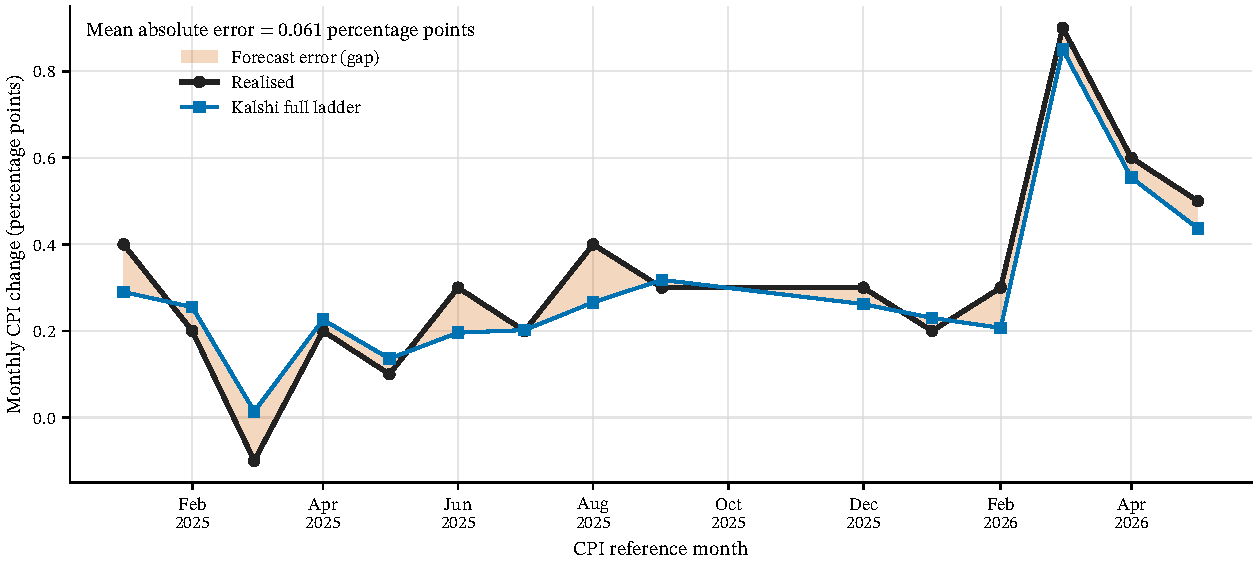
\includegraphics[width=0.88\textwidth]{figures/cpi_h1_kalshi_forecast_error_band.pdf}
\caption{Terminal full-ladder Kalshi forecast and realised month-over-month
CPI inflation, 15 test events. Shading is the forecast error.}
\label{fig:cpi-errorband}
\end{figure}

Figure~\ref{fig:cpi-errorband} identifies the largest CPI errors. Absolute
errors exceed 0.10 percentage points in August 2025 (0.27 forecast, 0.40
realised), March 2025 (0.01, $-0.10$), January 2025 (0.29, 0.40), and June 2025
(0.20, 0.30). March 2026 has the largest realised value, 0.90, and a forecast
of 0.85. Three of the four largest errors are underforecasts. The mean signed
error is $-0.024$ percentage points, consistent with the H2 asymmetry.

Policy-rate MAE is 0.012 percentage points, less than one twentieth of a
25-basis-point policy step. The largest error occurs in March 2025, with a
forecast of 4.46 and outcome of 4.50. For the index, 10 of 229 errors exceed
100 points. The largest occurs on 28 November 2025, with a forecast of 6{,}621
and close of 6{,}849. Mean signed error is $-12.1$ points. The corresponding terminal full-ladder forecast-error plots for the policy
rate and the index are reported in
Appendix~\ref{app:forecast-error-figures},
Figures~\ref{fig:app-ffr-errorband} and~\ref{fig:app-sp500-errorband}.

H1a is supported for all targets on the primary reading, with adjusted
$p$-values from 0.005 to 0.043. This comparison shows that the market improves
on simple time-series baselines.




\subsection{Against the External Benchmarks (H1b)}
\label{sec:results-h1b}
\label{sec:results-sp500-h1b}

\begin{table}[htbp]
\centering
\caption{H1b: Accuracy against External Benchmarks}
\label{tab:h1b}
\small
\begin{tabular}{@{}llrrrrrl@{}}
\toprule
Target & Benchmark & $N$ & Kalshi & Bench. & $\Delta$ & DM & $p$ \\
\midrule
CPI (pp) & Cleveland nowcast & 15 & 0.0725 & 0.0839 & $0.0114$ & 0.88 & 0.394 \\
FFR (pp) & Fed funds futures & 12 & 0.0155 & 0.0146 & $-0.0009$ & $-0.17$ & 0.869 \\
S\&P (index pts) & E-mini futures & 158 & 48.58 & 20.74 & $-27.85$ & $-4.44$ & $<0.001$ \\
\midrule
\multicolumn{8}{@{}l}{\emph{Sensitivity: the same comparison on the top-3 reading}} \\
S\&P (index pts) & E-mini futures & 158 & 21.68 & 20.74 & $-0.94$ & $-0.42$ & 0.672 \\
\bottomrule
\end{tabular}
\tablenote{The Kalshi mean is compared with each target's external benchmark
on the exact common sample. $\Delta$ is the benchmark RMSE minus the Kalshi
RMSE, so positive favours the market. The final row is sensitivity evidence,
not a second test of the hypothesis.}
\end{table}

External benchmark results differ by target.

The CPI bootstrap interval is $[-0.012,\ 0.036]$.

For the policy rate, the interval is $[-0.012,\ 0.008]$.

The primary index interval is $[-37.24,\ -19.21]$.

For the top-3 reading, it is $[-5.20,\ 3.48]$.

For CPI, Kalshi RMSE is lower by 0.0114 percentage points, about 14~percent of
the nowcast error, but the interval includes zero. The comparison is
inconclusive. The Cleveland nowcast \parencite{knotek2017} remains much more
accurate than the AR(3), with RMSE 0.0839 rather than 0.2480.

For the policy rate, federal funds futures have RMSE 0.0146 and Kalshi has
0.0155. The difference is 0.0009 percentage points, less than one tenth of a
basis point, and cannot be resolved with twelve meetings. The established
futures market \parencite{gurkaynak2007} and Kalshi therefore produce similar
point estimates, but the test does not establish equivalence. The futures risk
premium remains unadjusted as described in Section~\ref{sec:benchmarks}.

For the index, H1b is rejected in favour of the futures benchmark. On 158
common days, futures RMSE is 20.74 and full-ladder RMSE is 48.58. The benchmark
error is 57~percent lower, the bootstrap interval excludes zero, and the DM
statistic is $-4.44$. Serial dependence described in
Section~\ref{sec:results-design-accuracy} may affect the reported precision but
is unlikely to reverse this large difference. The $p$-value should not be read
at nominal precision. Table~\ref{tab:h1b} reports the comparison.

The top-3 sensitivity measure has RMSE 21.68, compared with 20.74 for futures,
and the difference is inconclusive. Across all 229 days, full-ladder and top-3
RMSE values are 46.51 and 24.98; median absolute errors are 18.8 and 7.0 points.
The full ladder underpredicts the close by 12.1 points on average, while the
top-3 mean overpredicts by 0.7 points. An index event has a median of ten traded
brackets, and outer brackets may become stale as the underlying moves. Their
inclusion can lower the full-ladder estimate in a rising market.

The full ladder remains the prespecified primary measure. The primary result
is therefore that Kalshi is less accurate than the futures benchmark for the
index. The top-3 result is sensitivity evidence that the aggregation rule
contributes to the difference.

H1b is inconclusive for CPI and the policy rate and rejected in favour of the
external benchmark for the index. The two inconclusive results do not
demonstrate equal accuracy.

\subsection{Against the Trained Models (H1c)}
\label{sec:results-h1c}

H1c asks whether any trained model attains lower out-of-sample error than the
Kalshi implied mean. Each target has six model configurations under the
terminal, unweighted and weighted training designs, producing eighteen runs.
The stochastic forecasts are five-seed ensembles. Tables~\ref{tab:h1c-cpi}--
\ref{tab:h1c-sp500} report every run alongside the market readings and
benchmarks.

The Diebold--Mariano statistics compare each row with the full-ladder Kalshi
mean. A positive statistic favours Kalshi and a negative statistic favours the
forecast in that row. The displayed $p$-values are two-sided and unadjusted,
allowing the individual comparisons to be read directly. The hypothesis
verdicts in the text use Holm adjustment across each target's pooled competitor
set.

% Source:
% Reproducibility/CPI/results/cpi_models_metrics.csv
% Reproducibility/CPI/results/cpi_significance_tests.csv
\begin{table}[H]
\centering
\caption{H1c: CPI Forecast Accuracy}
\label{tab:h1c-cpi}
\footnotesize
\begin{tabular}{@{}llrrrr@{}}
\toprule
Group & Forecast & RMSE & MAE & DM & $p$ \\
\midrule
Market & Kalshi, top 3 & 0.068 & 0.058 & $-1.27$ & 0.224 \\
 & Kalshi, full ladder & 0.072 & 0.061 & -- & -- \\
\midrule
External & Cleveland nowcast & 0.084 & 0.072 & 0.88 & 0.394 \\
\midrule
Baseline & AR(3) & 0.248 & 0.204 & 2.62 & 0.020 \\
\midrule
Terminal & GBM, Kalshi & 0.131 & 0.106 & 2.73 & 0.016 \\
 & GBM, hybrid & 0.135 & 0.105 & 1.66 & 0.119 \\
 & LSTM, Kalshi & 0.145 & 0.124 & 3.18 & 0.007 \\
 & LSTM, hybrid & 0.181 & 0.151 & 2.57 & 0.022 \\
 & MLP, history & 0.226 & 0.164 & 1.75 & 0.102 \\
 & GBM, history & 0.248 & 0.178 & 1.67 & 0.117 \\
\midrule
Unweighted & GBM, Kalshi & 0.095 & 0.079 & 1.23 & 0.238 \\
 & LSTM, Kalshi & 0.150 & 0.121 & 2.39 & 0.031 \\
 & LSTM, hybrid & 0.154 & 0.124 & 2.31 & 0.037 \\
 & GBM, hybrid & 0.200 & 0.138 & 1.41 & 0.182 \\
 & MLP, history & 0.213 & 0.162 & 2.05 & 0.060 \\
 & GBM, history & 0.247 & 0.167 & 1.58 & 0.137 \\
\midrule
Weighted & GBM, Kalshi & 0.094 & 0.075 & 0.85 & 0.410 \\
 & LSTM, Kalshi & 0.105 & 0.085 & 1.44 & 0.172 \\
 & LSTM, hybrid & 0.149 & 0.124 & 2.56 & 0.023 \\
 & GBM, hybrid & 0.173 & 0.129 & 1.65 & 0.121 \\
 & MLP, history & 0.213 & 0.169 & 2.21 & 0.044 \\
 & GBM, history & 0.244 & 0.175 & 1.66 & 0.120 \\
\bottomrule
\end{tabular}
\tablenote{Forecast comparison for CPI over the 15 test releases. Errors are
in percentage points. DM statistics compare each forecast with the full-ladder
Kalshi mean; $p$-values are two-sided and unadjusted.}
\end{table}

Table~\ref{tab:h1c-cpi} shows that no trained CPI model improves on either
market reading. The full-ladder and top-3 RMSE values are 0.072 and 0.068,
respectively. The best trained model is the weighted Kalshi-input GBM, with
RMSE 0.094, about 30~percent above the full-ladder value. Its two-sided
$p$-value is 0.410.

The Kalshi-input GBM improves from RMSE 0.131 under terminal training to 0.095
under unweighted training and 0.094 under weighted training. Although several
individual rows have unadjusted $p$-values below 0.05, none of the eighteen
model comparisons remains significant after pooled Holm adjustment. H1c is
therefore supported for CPI: none of the tested models attains lower error than
the market.

% Source:
% Reproducibility/FFR/results/ffr_models_metrics.csv
% Reproducibility/FFR/results/ffr_significance_tests.csv
\begin{table}[H]
\centering
\caption{H1c: Federal Funds Rate Forecast Accuracy}
\label{tab:h1c-ffr}
\footnotesize
\begin{tabular}{@{}llrrrr@{}}
\toprule
Group & Forecast & RMSE & MAE & DM & $p$ \\
\midrule
Market & Kalshi, full ladder & 0.0155 & 0.0119 & -- & -- \\
 & Kalshi, top 3 & 0.0718 & 0.0260 & 0.96 & 0.358 \\
\midrule
External & Fed funds futures & 0.0146 & 0.0100 & $-0.17$ & 0.869 \\
\midrule
Baseline & No-change rule & 0.1250 & 0.0625 & 1.88 & 0.087 \\
 & AR(3) & 0.1496 & 0.1195 & 2.75 & 0.019 \\
\midrule
Terminal & GBM, history & 0.2150 & 0.1360 & 1.95 & 0.077 \\
 & GBM, Kalshi & 0.2635 & 0.1916 & 2.42 & 0.034 \\
 & GBM, hybrid & 0.3124 & 0.2117 & 1.66 & 0.125 \\
 & LSTM, Kalshi & 0.7989 & 0.5361 & 1.53 & 0.154 \\
 & LSTM, hybrid & 1.3068 & 1.0104 & 2.22 & 0.048 \\
 & MLP, history & 1.5256 & 1.3381 & 3.79 & 0.003 \\
\midrule
Unweighted & GBM, Kalshi & 0.1954 & 0.1255 & 1.96 & 0.075 \\
 & LSTM, Kalshi & 0.2051 & 0.1470 & 2.16 & 0.053 \\
 & GBM, history & 0.2207 & 0.1368 & 1.85 & 0.092 \\
 & GBM, hybrid & 0.2403 & 0.1602 & 2.08 & 0.062 \\
 & LSTM, hybrid & 0.5285 & 0.3798 & 1.64 & 0.130 \\
 & MLP, history & 1.0817 & 0.9648 & 4.32 & 0.001 \\
\midrule
Weighted & GBM, Kalshi & 0.1640 & 0.1106 & 2.59 & 0.025 \\
 & GBM, history & 0.2185 & 0.1354 & 1.88 & 0.087 \\
 & GBM, hybrid & 0.2372 & 0.1520 & 2.01 & 0.070 \\
 & LSTM, Kalshi & 0.2471 & 0.1635 & 1.34 & 0.206 \\
 & LSTM, hybrid & 0.6686 & 0.4628 & 1.56 & 0.148 \\
 & MLP, history & 0.7204 & 0.6477 & 3.76 & 0.003 \\
\bottomrule
\end{tabular}
\tablenote{Forecast comparison for the federal funds rate over the 12 test
meetings. Errors are in percentage points. DM statistics compare each forecast
with the full-ladder Kalshi mean; $p$-values are two-sided and unadjusted.}
\end{table}

Table~\ref{tab:h1c-ffr} shows a larger separation between the market and the
trained models. The full-ladder market RMSE is 0.0155, while the best model,
the weighted Kalshi-input GBM, has RMSE 0.1640. It therefore has more than ten
times the error of the primary market reading.

The Kalshi-input GBM improves from 0.2635 under terminal training to 0.1954
under unweighted training and 0.1640 under weighted training, but remains far
behind the market under every design. Six model rows are significantly worse
before adjustment, but only one survives pooled Holm adjustment. For example,
the weighted Kalshi-input LSTM has RMSE 0.2471 but an unadjusted $p$-value of
0.206. With only twelve meetings, a few large errors generate substantial
variation in the loss differential. H1c is supported for the policy rate
because no trained model improves on either market reading.

% Source:
% Reproducibility/SP500/results/sp500_models_metrics.csv
% Reproducibility/SP500/results/sp500_significance_tests.csv
% The futures row uses the matched 158-day sample.
\begin{table}[H]
\centering
\caption{H1c: S\&P~500 Forecast Accuracy}
\label{tab:h1c-sp500}
\footnotesize
\begin{tabular}{@{}llrrrr@{}}
\toprule
Group & Forecast & RMSE & MAE & DM & $p$ \\
\midrule
Market & Kalshi, top 3 & 24.98 & 14.04 & $-4.20$ & $<0.001$ \\
 & Kalshi, full ladder & 46.51 & 31.61 & -- & -- \\
\midrule
External & S\&P 500 futures (158 days) & 20.74 & 14.58 & $-4.44$ & $<0.001$ \\
\midrule
Baseline & AR(3) & 59.40 & 45.56 & 2.81 & 0.005 \\
 & Previous close & 59.62 & 45.57 & 2.85 & 0.005 \\
\midrule
Terminal & GBM, hybrid & 26.85 & 18.47 & $-3.99$ & $<0.001$ \\
 & LSTM, hybrid & 26.98 & 18.66 & $-4.02$ & $<0.001$ \\
 & GBM, Kalshi & 27.40 & 18.73 & $-3.86$ & $<0.001$ \\
 & LSTM, Kalshi & 27.98 & 18.71 & $-3.74$ & $<0.001$ \\
 & MLP, history & 60.46 & 46.30 & 2.99 & 0.003 \\
 & GBM, history & 62.37 & 47.74 & 3.09 & 0.002 \\
\midrule
Unweighted & LSTM, Kalshi & 30.09 & 20.72 & $-3.42$ & 0.001 \\
 & LSTM, hybrid & 32.05 & 23.09 & $-3.14$ & 0.002 \\
 & GBM, Kalshi & 33.29 & 24.15 & $-2.86$ & 0.005 \\
 & GBM, hybrid & 43.83 & 30.30 & $-0.56$ & 0.575 \\
 & MLP, history & 60.29 & 46.67 & 3.02 & 0.003 \\
 & GBM, history & 63.69 & 47.72 & 3.21 & 0.001 \\
\midrule
Weighted & LSTM, Kalshi & 27.64 & 18.74 & $-3.84$ & $<0.001$ \\
 & LSTM, hybrid & 30.66 & 21.73 & $-3.36$ & 0.001 \\
 & GBM, Kalshi & 31.83 & 22.48 & $-3.12$ & 0.002 \\
 & GBM, hybrid & 38.88 & 26.57 & $-1.63$ & 0.104 \\
 & MLP, history & 60.50 & 46.62 & 3.04 & 0.003 \\
 & GBM, history & 63.90 & 47.77 & 3.21 & 0.002 \\
\bottomrule
\end{tabular}
\tablenote{Forecast comparison for the S\&P~500 over the 229 test days.
Errors are in index points. The futures row uses the 158 futures-covered days
and is not directly comparable with the remaining RMSE and MAE rows. DM
statistics compare each forecast with the full-ladder Kalshi mean on the
relevant common sample; $p$-values are two-sided and unadjusted.}
\end{table}

Table~\ref{tab:h1c-sp500} produces a different conclusion. Twelve of the
eighteen trained models have lower RMSE than the primary full-ladder mean, and
ten of these improvements remain significant after pooled Holm adjustment. The
best run is the terminal hybrid GBM, with RMSE 26.85 compared with 46.51 for
the full ladder.

All twelve models that improve on the full ladder use Kalshi price-path inputs.
The six history-only models have RMSE values between 60.29 and 63.90 and are
significantly worse. Market prices therefore contain the information that
allows the trained models to improve on the full-ladder forecast.

No model improves on the top-3 RMSE of 24.98. The best trained model has
approximately 7~percent higher error. Models can improve on a full-ladder mean
affected by stale outer brackets, but not on the three high-volume brackets
that form their own market input. The index models are refitted monthly, so
their parameters can be almost one month old; this feature favours the
continuously updating market. Three of the four best runs use terminal
training, suggesting that excluding distant windows is more useful than
retaining the full intraday history for this target.

% Source:
% Reproducibility/SP500/results/sp500_models_metrics_returns.csv
% Reproducibility/SP500/results/sp500_models_metrics_returns_with_futures.csv
% The futures row uses the matched 158-day sample.
\begin{table}[htbp]
\centering
\caption{H1c: S\&P~500 Forecast Accuracy in Log Returns}
\label{tab:h1c-sp500-returns}
\footnotesize
\begin{tabular}{@{}llrrrr@{}}
\toprule
Group & Forecast & RMSE (\%) & MAE (\%) & DM & $p$ \\
\midrule
Market & Kalshi, top 3 & 0.401 & 0.220 & $-3.81$ & $<0.001$ \\
 & Kalshi, full ladder & 0.719 & 0.484 & -- & -- \\
\midrule
External & S\&P 500 futures (158 days) & 0.298 & 0.210 & $-4.40$ & $<0.001$ \\
\midrule
Baseline & AR(3) & 0.913 & 0.697 & 2.67 & 0.008 \\
 & Previous close & 0.919 & 0.698 & 2.75 & 0.006 \\
\midrule
Terminal & GBM, hybrid & 0.432 & 0.288 & $-3.62$ & $<0.001$ \\
Unweighted & LSTM, Kalshi & 0.477 & 0.320 & $-3.12$ & 0.002 \\
Weighted & LSTM, Kalshi & 0.444 & 0.292 & $-3.49$ & 0.001 \\
\bottomrule
\end{tabular}
\tablenote{Selected forecast comparison for the S\&P~500 in log-return units.
Errors are multiplied by 100 and can be read as approximate
percentage returns. The table shows both market readings, the external
benchmark, the prespecified baselines, and the lowest-RMSE trained model from
each design. The futures row uses 158 common days; all other rows use 229 days.
DM statistics compare each forecast with the full-ladder Kalshi mean on the
relevant sample; $p$-values are two-sided and unadjusted.}
\end{table}

Table~\ref{tab:h1c-sp500-returns} shows that expressing errors as returns does
not change the ranking. Full-ladder RMSE is 0.719~percent, compared with
0.919~percent for the previous-close rule and 0.913~percent for AR(3). The
top-3 reading has RMSE 0.401~percent. The best model under each training design
has lower RMSE than the full ladder, between 0.432 and 0.477~percent, with
two-sided unadjusted $p$-values no greater than 0.002. None improves on the
top-3 reading by raw RMSE. On the 158 days covered by the futures series,
futures have the lowest displayed RMSE at 0.298~percent. The return-space
evidence therefore confirms that the gains in Table~\ref{tab:h1c-sp500} are
not caused solely by changes in the nominal index level.

H1c is therefore supported for CPI and the policy rate and rejected for the
S\&P~500 on the prespecified full-ladder reading. This conclusion is restricted
to the six model configurations, three training designs and stated S\&P~500
refit cadence.


\section{Distributional Calibration across Targets}
\label{sec:results-h2}

\begin{table}[htbp]
\centering
\caption{H2: Distributional Calibration}
\label{tab:h2}
\small
\begin{tabular}{@{}lrrrrrrrr@{}}
\toprule
 & & \multicolumn{2}{c}{Uniformity} & \multicolumn{2}{c}{Tail share}
 & \multicolumn{3}{c}{Central coverage} \\
\cmidrule(lr){3-4}\cmidrule(lr){5-6}\cmidrule(lr){7-9}
Target & $N$ & KS & CvM & Lower & Upper & 50\% & 80\% & 90\% \\
\midrule
CPI & 45 & 0.332$^\dagger$ & 2.186$^\dagger$ & 0.022 & 0.289$^\dagger$
 & 0.489 & 0.689 & 0.778$^\dagger$ \\
FFR & 35 & 0.094 & 0.041 & 0.114 & 0.057
 & 1.000$^\dagger$ & 1.000$^\dagger$ & 1.000 \\
S\&P 500 & 859 & 0.067$^\dagger$ & 1.224$^\dagger$ & 0.056$^\dagger$ & 0.056$^\dagger$
 & 0.863$^\dagger$ & 0.952$^\dagger$ & 0.983$^\dagger$ \\
\bottomrule
\end{tabular}
\tablenote{Calibration of the terminal implied distribution for all labelled
events. The S\&P~500 ladder is read at the two-hour pre-close window. Tail
shares have an expected value of 0.10 and coverage rates 0.50, 0.80 and 0.90.
Holm adjusts across the seven tests within a target; $\dagger$ marks a
rejection at the 5~percent level after adjustment.}
\end{table}

H2 is rejected for CPI and the S\&P~500. Uniformity and tail tests do not reject
for the policy rate. Table~\ref{tab:h2} shows that the CPI and equity failures
have opposite directions.

\begin{figure}[htbp]
\centering
\begin{minipage}{0.49\textwidth}
\centering
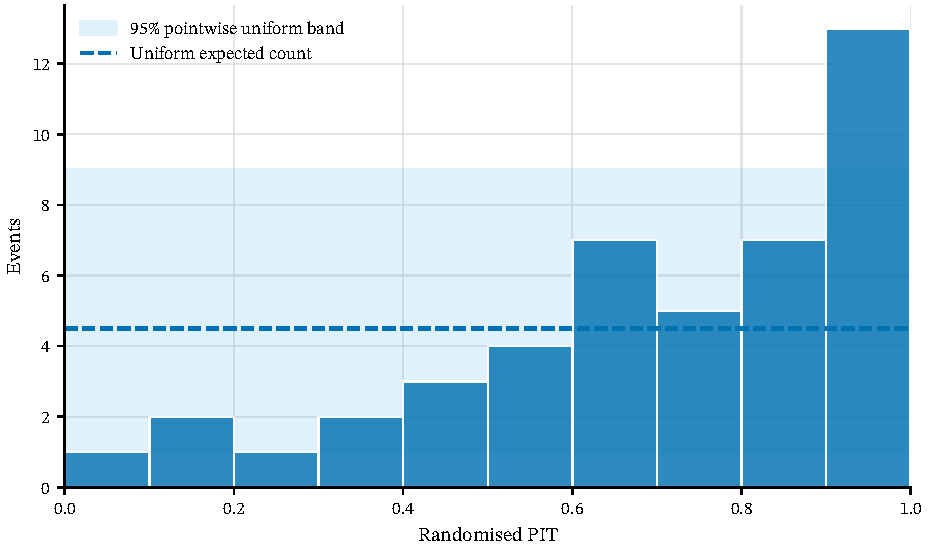
\includegraphics[width=\textwidth]{figures/cpi_h2_pit_histogram.pdf}
\end{minipage}
\hfill
\begin{minipage}{0.49\textwidth}
\centering
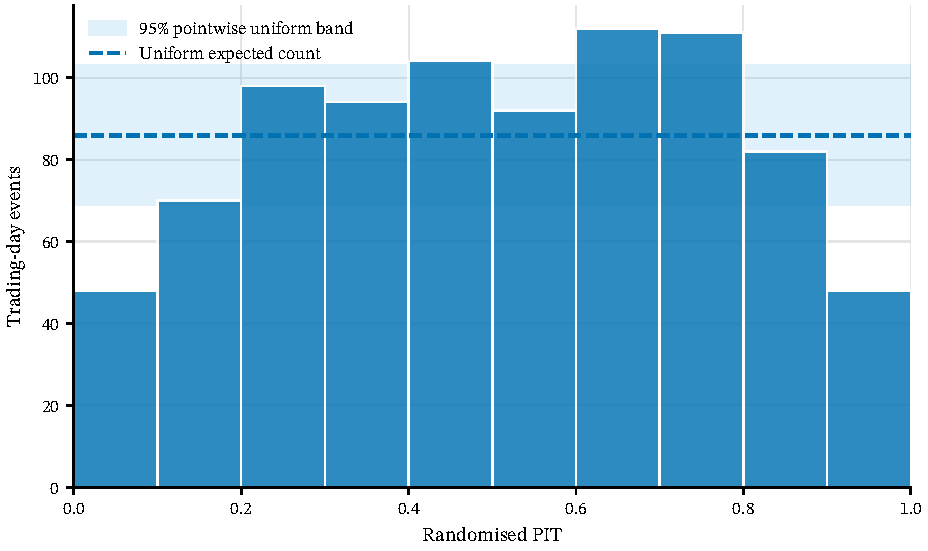
\includegraphics[width=\textwidth]{figures/sp500_h2_pit_histogram.pdf}
\end{minipage}
\caption{Randomised PIT values: 45 CPI releases (left) and 859 trading days
(right). The dashed line is the count a calibrated ladder would produce and
the band is a 95~percent pointwise interval around it.}
\label{fig:pit}
\end{figure}

The CPI ladder is too narrow in the upper tail. The share above the implied
90th percentile is 28.9~percent rather than 10~percent, while the lower-tail
share is 2.2~percent. The 90~percent interval covers 77.8~percent of events,
but 50~percent coverage is close to nominal at 48.9~percent. In the left
panel of Figure~\ref{fig:pit}, the final bin contains 13 of 45 observations.
Risk premia and longshot overpricing would widen priced tails, while this
result shows an upper tail that is too narrow, as discussed in
Section~\ref{sec:results-design-pit}. Uniformity is rejected for all
500 randomisation seeds, and the upper-tail share ranges from 0.178 to 0.400.

The index distribution is too wide. Each tail contains 5.6~percent of closes
rather than 10~percent. Coverage is 86.3, 95.2, and 98.3~percent for nominal
50, 80, and 90~percent intervals. The right panel of Figure~\ref{fig:pit} is
centred and hump-shaped, with mean PIT 0.510 and 48 observations in each end
bin. Risk premia and longshot overpricing are consistent with this direction
because they add probability to distant brackets. Uniformity is rejected for
all 500 seeds, with tail shares between 0.040 and 0.078. The KS statistic is
0.067 and is precisely estimated because the sample contains 859 events; the large coverage excesses
show the economic magnitude.

\begin{figure}[htbp]
\centering
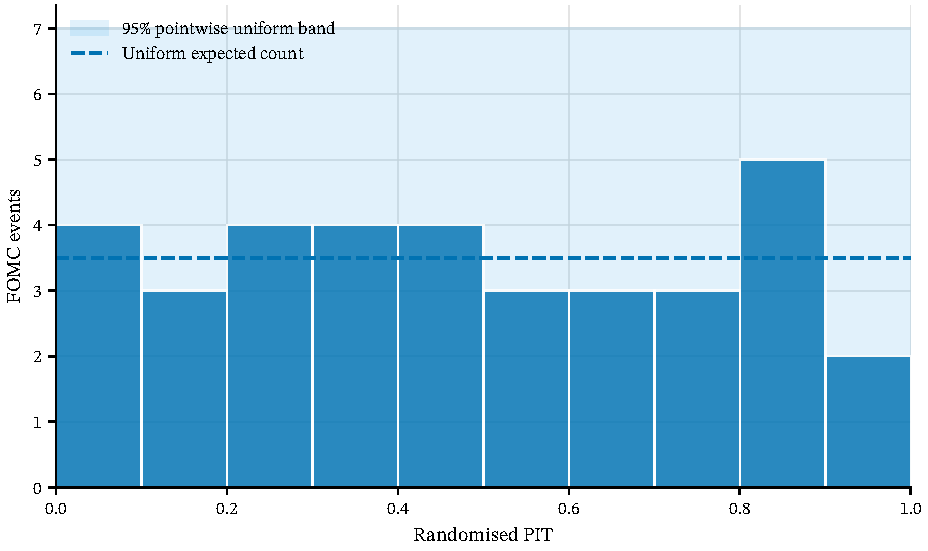
\includegraphics[width=0.6\textwidth]
{figures/ffr_h2_pit_histogram.pdf}
\caption{Randomised PIT values for 35 policy-rate decisions. The dashed line
is the expected count under a uniform distribution.}
\label{fig:ffr-pit}
\end{figure}

The policy-rate case is affected by discreteness. Figure~\ref{fig:ffr-pit}
shows that the PIT histogram appears approximately uniform, but this result
requires caution. Uniformity and tail tests do not reject, while all three
central intervals have 100~percent coverage. The distribution assigns a mean
probability of 0.913 and a median probability of 0.95 to the realised outcome;
30 of 35 distributions assign it more than 0.90. September 2024 is the main
exception, when a 50-basis-point cut had probability 0.30. When one outcome has
most of the mass, randomisation spreads the PIT over much of the unit interval
and reduces test power. Central intervals also collapse to the dominant
outcome, so their 100~percent
coverage does not imply excessive width. Across 500 seeds, the KS test rejects
19 times and the CvM test 26 times. Non-rejection is common but not universal.

H2 therefore fails for CPI and the index. It is not rejected for policy-rate
uniformity or tails, but the tests are weakly informative and do not establish
calibration. All results concern marginal distributions because serial
independence is untested. Point accuracy and calibration remain distinct: the
CPI centre is accurate but its upper tail is too narrow, while the index
distribution is too wide.

\section{Incremental Information across Targets}
\label{sec:results-h3}

The information-set results are reported in two stages. Table~\ref{tab:h3}
summarises the direction and significance of the comparisons across targets,
while Table~\ref{tab:h3pairs} reports the underlying matched RMSE pairs.

\begin{table}[H]
\centering
\caption{H3: Information-Set Results}
\label{tab:h3}
\small
\begin{tabular}{@{}llrrrr@{}}
\toprule
 & Target & Predicted direction & Bootstrap excludes 0 & Raw $p<0.05$ & Survives Holm \\
\midrule
H3a & CPI & 6 & 3 & 1 & 0 \\
 & FFR & 5 & 3 & 3 & 2 \\
 & S\&P 500 & 6 & 6 & 6 & 6 \\
\midrule
H3b & CPI & 6 & 2 & 1 & 0 \\
 & FFR & 6 & 2 & 1 & 0 \\
 & S\&P 500 & 4 & 3 & 3 & 3 \\
\bottomrule
\end{tabular}
\tablenote{Matched comparisons between information sets for H3a and H3b, six
per hypothesis per target. Two models enter a pair only if they share a model
type and a training design. Counts are out of six; ``Holm'' applies within
each hypothesis and target.}
\end{table}

Table~\ref{tab:h3} shows that the predicted H3a direction holds in 17 of 18
matched pairs and that the predicted H3b direction holds in 16 of 18 pairs.
Holm-adjusted support is strongest for the S\&P~500, while fewer comparisons
survive adjustment for the two macroeconomic targets.

\begin{table}[htbp]
\centering
\caption{H3: Matched Information-Set Comparisons}
\label{tab:h3pairs}
\small
\begin{tabular}{@{}llrrrl@{}}
\toprule
Model & Design & Market & Other & $\Delta$ & 95\% bootstrap \\
\midrule
\multicolumn{6}{@{}l}{\emph{CPI --- H3a: market against history only}} \\
GBM & Terminal & 0.1308 & 0.2478 & 0.1170 & $[-0.013,\ 0.254]$ \\
 & Unweighted & 0.0947 & 0.2470 & 0.1523 & $[\phantom{-}0.011,\ 0.278]$ \\
 & Weighted & 0.0935 & 0.2443 & 0.1508 & $[\phantom{-}0.031,\ 0.257]$ \\
Neural & Terminal & 0.1446 & 0.2259 & 0.0814 & $[-0.022,\ 0.174]$ \\
 & Unweighted & 0.1501 & 0.2134 & 0.0634 & $[-0.025,\ 0.140]$ \\
 & Weighted & 0.1055 & 0.2129 & 0.1074 & $[\phantom{-}0.042,\ 0.158]$ \\
\multicolumn{6}{@{}l}{\emph{CPI --- H3b: market against hybrid}} \\
GBM & Terminal & 0.1308 & 0.1345 & 0.0037 & $[-0.049,\ 0.048]$ \\
 & Unweighted & 0.0947 & 0.2000 & 0.1053 & $[-0.006,\ 0.211]$ \\
 & Weighted & 0.0935 & 0.1726 & 0.0791 & $[\phantom{-}0.004,\ 0.144]$ \\
Neural & Terminal & 0.1446 & 0.1814 & 0.0368 & $[-0.011,\ 0.081]$ \\
 & Unweighted & 0.1501 & 0.1540 & 0.0040 & $[-0.027,\ 0.032]$ \\
 & Weighted & 0.1055 & 0.1488 & 0.0433 & $[\phantom{-}0.001,\ 0.084]$ \\
\midrule
\multicolumn{6}{@{}l}{\emph{FFR --- H3a: market against history only}} \\
GBM & Terminal & 0.2635 & 0.2150 & $-0.0486$ & $[-0.189,\ 0.089]$ \\
 & Unweighted & 0.1954 & 0.2207 & 0.0253 & $[-0.132,\ 0.180]$ \\
 & Weighted & 0.1640 & 0.2185 & 0.0544 & $[-0.071,\ 0.184]$ \\
Neural & Terminal & 0.7989 & 1.5256 & 0.7267 & $[\phantom{-}0.121,\ 1.407]$ \\
 & Unweighted & 0.2051 & 1.0817 & 0.8766 & $[\phantom{-}0.578,\ 1.140]$ \\
 & Weighted & 0.2471 & 0.7204 & 0.4733 & $[\phantom{-}0.196,\ 0.753]$ \\
\multicolumn{6}{@{}l}{\emph{FFR --- H3b: market against hybrid}} \\
GBM & Terminal & 0.2635 & 0.3124 & 0.0489 & $[-0.122,\ 0.246]$ \\
 & Unweighted & 0.1954 & 0.2403 & 0.0449 & $[-0.114,\ 0.195]$ \\
 & Weighted & 0.1640 & 0.2372 & 0.0732 & $[-0.061,\ 0.199]$ \\
Neural & Terminal & 0.7989 & 1.3068 & 0.5078 & $[\phantom{-}0.291,\ 0.777]$ \\
 & Unweighted & 0.2051 & 0.5285 & 0.3234 & $[-0.006,\ 0.633]$ \\
 & Weighted & 0.2471 & 0.6686 & 0.4215 & $[\phantom{-}0.172,\ 0.642]$ \\
\midrule
\multicolumn{6}{@{}l}{\emph{S\&P 500 --- H3a: market against history only}} \\
GBM & Terminal & 27.40 & 62.37 & 34.96 & $[\phantom{-}27.63,\ 42.46]$ \\
 & Unweighted & 33.29 & 63.69 & 30.40 & $[\phantom{-}23.96,\ 37.24]$ \\
 & Weighted & 31.83 & 63.90 & 32.06 & $[\phantom{-}25.63,\ 39.25]$ \\
Neural & Terminal & 27.98 & 60.46 & 32.48 & $[\phantom{-}25.85,\ 39.28]$ \\
 & Unweighted & 30.09 & 60.29 & 30.19 & $[\phantom{-}24.60,\ 35.72]$ \\
 & Weighted & 27.64 & 60.50 & 32.85 & $[\phantom{-}27.03,\ 38.88]$ \\
\multicolumn{6}{@{}l}{\emph{S\&P 500 --- H3b: market against hybrid}} \\
GBM & Terminal & 27.40 & 26.85 & $-0.55$ & $[-3.15,\ 1.84]$ \\
 & Unweighted & 33.29 & 43.83 & 10.54 & $[\phantom{-}5.70,\ 15.94]$ \\
 & Weighted & 31.83 & 38.88 & 7.04 & $[\phantom{-}3.29,\ 11.49]$ \\
Neural & Terminal & 27.98 & 26.98 & $-1.00$ & $[-2.69,\ 0.77]$ \\
 & Unweighted & 30.09 & 32.05 & 1.95 & $[-0.48,\ 4.55]$ \\
 & Weighted & 27.64 & 30.66 & 3.02 & $[\phantom{-}0.91,\ 5.40]$ \\
\bottomrule
\end{tabular}
\tablenote{The 36 matched pairs behind Table~\ref{tab:h3}. ``Market'' is the
Kalshi-input model and ``other'' its history-only counterpart under H3a or its
hybrid counterpart under H3b. $\Delta$ is other minus market, so positive
supports the hypothesis. Units are percentage points for the CPI and FFR and
index points for the S\&P~500; intervals are 95~percent event bootstraps.}
\end{table}

H3a compares market-input and history-only models. Table~\ref{tab:h3pairs}
reports the pairs summarised in Table~\ref{tab:h3}. The exception to the
predicted direction is the terminal policy-rate GBM, where
market-input RMSE is 0.2635 and history-only RMSE is 0.2150. This pair has at
most 34 training rows, and the policy rate is a step function that is often
easy to extrapolate over short periods. Across designs, the history-only GBM
has RMSE 0.2150--0.2207, while the simpler AR(3) reaches 0.1496.

For the index, market-input models have RMSE 27.64--33.29, compared with
60.29--63.90 for history-only models. All six pairs survive Holm adjustment
with $p$ below 0.001. For CPI, the weighted comparison is 0.0935 against 0.2443, but
only one pair is significant before adjustment and none after Holm correction.
For the policy rate, two neural pairs survive, with $p = 0.006$ and $p = 0.036$.
The history MLP has RMSE 0.7204--1.5256, while all GBM intervals include zero
and differences range from $-0.0486$ to $0.0544$.

H3b tests whether target history improves a model that already uses market
prices. For CPI and the policy rate, all twelve hybrid models are worse than
their market-only counterparts. Under full-window training, CPI hybrid GBM
RMSE rises from 0.0947 to 0.2000 and from 0.0935 to 0.1726. Policy-rate hybrid
LSTM RMSE rises from 0.2051 to 0.5285 and from 0.2471 to 0.6686. Additional
lags increase model dimension without providing enough independent events.

For the index, market-only models win all four full-window comparisons and
three survive Holm adjustment. The hybrid GBM loses 10.54 points under
unweighted training and 7.04 under weighted training. Under terminal training,
the hybrid GBM and LSTM improve by 0.55 and 1.00 points, but neither difference
is significant; their adjusted $p$-values are 1.000 and both bootstrap
intervals include zero. Repeated history
features add no new information across windows within the same day.

H3a and H3b are supported in direction for all targets, but inferential
strength differs with sample size. Both are significant after adjustment for
the index. For the policy rate, only the neural H3a pairs survive. No CPI pair
survives multiplicity correction despite large RMSE differences. Overall, the
price paths contain more useful information than target history for the tested
models.

\clearpage
\section{Horizon Evidence and Model Weighting}
\label{sec:results-h5}

\subsection{Error and Revisions over the Contract's Life (H5a)}
\label{sec:results-h5a}

\begin{table}[htbp]
\centering
\caption{H5a: Forecast Accuracy by Horizon}
\label{tab:h5a}
\small
\begin{tabular}{@{}lrrrrrrrrr@{}}
\toprule
\multicolumn{10}{@{}l}{\emph{CPI, hours before release}} \\
 & 480 & 240 & 168 & 96 & 48 & 24 & 6 & & \\
RMSE & 0.0952 & 0.0851 & 0.0888 & 0.0826 & 0.0827 & 0.0818 & 0.0720 & & \\
Revision & 0.0368 & 0.0220 & 0.0227 & 0.0227 & 0.0161 & 0.0155 & 0.0108 & & \\
\midrule
\multicolumn{10}{@{}l}{\emph{FFR, hours before statement}} \\
 & 1440 & 720 & 480 & 240 & 168 & 96 & 48 & 24 & 6 \\
RMSE & 0.1278 & 0.0537 & 0.0508 & 0.0225 & 0.0228 & 0.0173 & 0.0172 & 0.0163 & 0.0157 \\
Revision & 0.0908 & 0.0387 & 0.0242 & 0.0073 & 0.0069 & 0.0038 & 0.0033 & 0.0021 & 0.0025 \\
\midrule
\multicolumn{10}{@{}l}{\emph{S\&P 500, hours before close}} \\
 & 36 & 24 & 12 & 6 & 4 & 2 & & & \\
RMSE & 98.69 & 99.51 & 95.79 & 69.74 & 59.60 & 51.86 & & & \\
Events & 101 & 106 & 121 & 214 & 226 & 229 & & & \\
\bottomrule
\end{tabular}
\tablenote{Full-ladder RMSE and mean absolute revision from the terminal
forecast at fixed pre-event cutoffs. Units are percentage points for the
first two targets and index points for the third. CPI and FFR cutoffs rest on
15 and 12 events throughout; the S\&P~500 event count is given in the table
because it falls with the horizon.}
\end{table}

Table~\ref{tab:h5a} shows that forecast errors and revisions generally decline
as each event approaches, but
none of the profiles is strictly monotonic. CPI RMSE rises from 0.0851 at 240
hours to 0.0888 at 168 hours and from 0.0826 at 96 hours to 0.0827 at 48 hours.
Policy-rate RMSE rises from 0.0225 at 240 hours to 0.0228 at 168 hours. Index
RMSE rises from 98.69 at 36 hours to 99.51 at 24 hours. H5a concerns the overall
profile and is supported for all targets.

The profiles differ in magnitude. Policy-rate RMSE falls from 0.1278 to
0.0157, mainly between 60 and 10 days before the statement. CPI RMSE changes
less, with the final value about one quarter below the starting error. Index
RMSE falls by about half within 36 hours. Revision measures show the same
ordering without using outcomes: policy-rate revisions decline from 0.0908 to
0.0025 percentage points, CPI revisions from 0.0368 to 0.0108, and index
revisions from 48.9 to 11.9 points on the futures-common sample.

For the index, the event count declines from 229 at two hours to 101 at 36
hours. Longer-horizon observations therefore cover only contracts that opened
early. The revision values and the following figure use the 158-day
futures-common sample, whereas the RMSE series above covers up to 229 days.
Chapter~\ref{ch:interpretation} uses the 229-day values for H5c.

\begin{figure}[H]
\centering
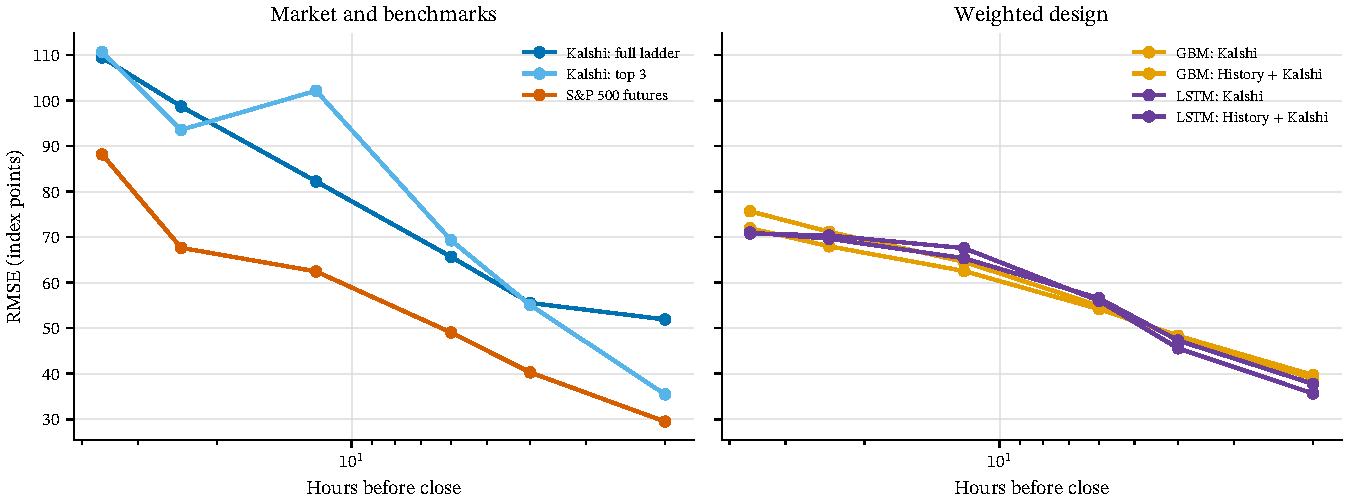
\includegraphics[width=0.92\textwidth]{figures/sp500_h5_model_rmse_by_forecast_horizon.pdf}
\caption{S\&P~500 RMSE by forecast horizon on the 158-day futures-common
sample: market readings and the futures benchmark (left), weighted-design
models (right). Event counts fall from 158 at two hours to 41 at 36.}
\label{fig:sp500-horizon}
\end{figure}

Figure~\ref{fig:sp500-horizon} extends H1 across the contract horizon. All four
model curves remain below the full-ladder curve at every cutoff and above the
futures curve except at 36 hours. The full ladder is more accurate at 6, 12,
and 36 hours, while the top-3 measure is more accurate within the final four
hours by 16.5 points. This pattern is consistent with Section~\ref{sec:results-h1b}:
late-session volume makes the most active brackets more current.

\begin{figure}[H]
\centering
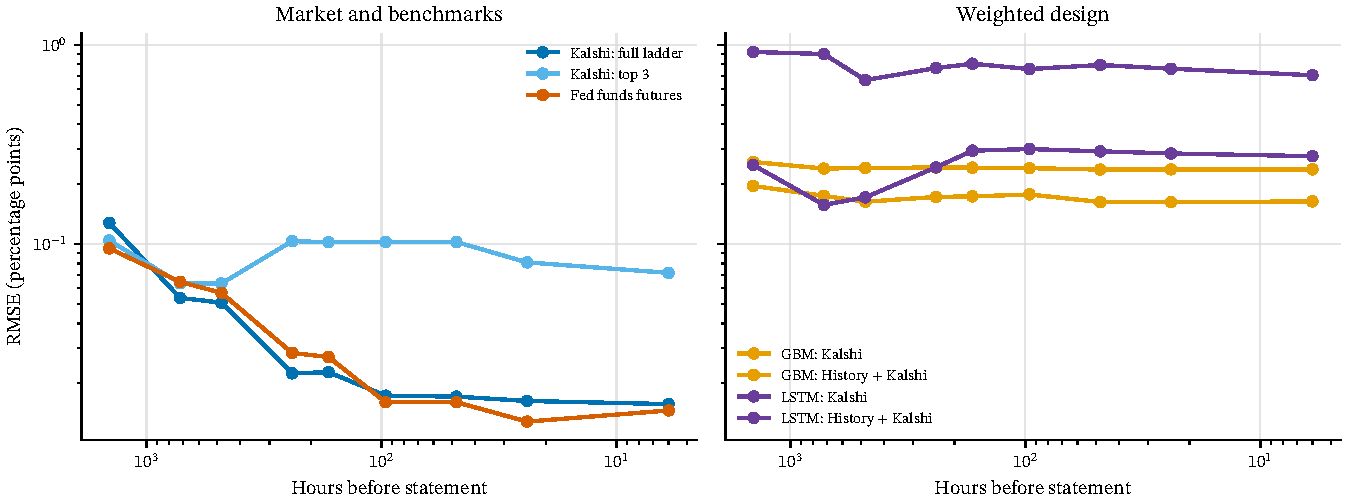
\includegraphics[width=0.92\textwidth]{figures/ffr_h5_model_rmse_by_forecast_horizon.pdf}
\caption{Federal funds rate RMSE by forecast horizon, 12 test meetings, on a
logarithmic vertical scale: market readings and the futures benchmark (left),
weighted-design models (right).}
\label{fig:ffr-horizon}
\end{figure}

Figure~\ref{fig:ffr-horizon} shows a different policy-rate pattern. Weighted
model RMSE remains between 0.16 and 0.92 percentage points at all horizons,
about an order of magnitude above the market readings, and does not decline
near the statement. The futures curve remains close to Kalshi. At 1{,}440
hours, futures RMSE is 0.0952 and Kalshi RMSE is 0.1278; futures is slightly
worse between 168 and 720 hours. The top-3 curve reaches 0.0634 at 480 hours,
rises to about 0.1035 between 240 and 48 hours, and ends at 0.0717. The April
2026 meeting explains much of this irregularity.

H5a is descriptive evidence of an overall decline for all targets. Forecast
error and remaining repricing decrease together as information arrives.

\subsection{Weighted against Unweighted Training (H5b)}
\label{sec:results-h5b}

\begin{table}[htbp]
\centering
\caption{H5b: Weighted versus Unweighted Training}
\label{tab:h5b}
\small
\begin{tabular}{@{}lrrrrrr@{}}
\toprule
 & \multicolumn{2}{c}{CPI} & \multicolumn{2}{c}{FFR}
 & \multicolumn{2}{c}{S\&P 500} \\
\cmidrule(lr){2-3}\cmidrule(lr){4-5}\cmidrule(lr){6-7}
Configuration & Unwt. & Wt. & Unwt. & Wt. & Unwt. & Wt. \\
\midrule
GBM, Kalshi & 0.0947 & 0.0935 & 0.1954 & 0.1640 & 33.29 & 31.83 \\
LSTM, Kalshi & 0.1501 & 0.1055 & 0.2051 & 0.2471 & 30.09 & 27.64 \\
GBM, hybrid & 0.2000 & 0.1726 & 0.2403 & 0.2372 & 43.83 & 38.88 \\
LSTM, hybrid & 0.1540 & 0.1488 & 0.5285 & 0.6686 & 32.05 & 30.66 \\
GBM, history & 0.2470 & 0.2443 & 0.2207 & 0.2185 & 63.69 & 63.90 \\
MLP, history & 0.2134 & 0.2129 & 1.0817 & 0.7204 & 60.29 & 60.50 \\
\midrule
Supporting H5b & \multicolumn{2}{c}{6/6} & \multicolumn{2}{c}{4/6}
 & \multicolumn{2}{c}{4/6} \\
\bottomrule
\end{tabular}
\tablenote{Terminal RMSE under the unweighted and weighted designs by
configuration. Units are percentage points for the CPI and FFR and index
points for the S\&P~500. A configuration supports H5b when the weighted value
is lower.}
\end{table}

As Table~\ref{tab:h5b} shows, weighting reduces terminal error in 14 of 18
configurations: 6 of 6 for CPI,
4 of 6 for the policy rate, and 4 of 6 for the index. H5b is fully supported
for CPI and partly supported for the other targets.

For the policy rate, weighting worsens the Kalshi-input and hybrid LSTMs. The
weighted Kalshi-input GBM is stable across seeds, with RMSE 0.16403--0.16404.
The Kalshi-input LSTM ranges from 0.244 to 0.392 under weighting and from 0.229
to 0.492 without weighting. These overlapping ranges show that the LSTM
ordering is within seed variation and cannot be resolved with twelve meetings.

For the index, weighting worsens only the two history-only configurations, by
less than 0.5~percent of their error. Every model using a market path improves;
the hybrid GBM declines from 43.83 to 38.88. However, terminal training is more
accurate than weighted training for five of six index configurations. For a
single-session contract, discarding distant windows may be more effective than
downweighting them.

H5b is a robustness test of the model design. Improvement in 14 of 18 cases is
evidence that the H5a horizon pattern is not solely an artefact of the
evaluation grid.

\clearpage
\section{Summary of Results}
\label{sec:results-summary}

\begin{table}[htbp]
\centering
\caption{Summary of Hypothesis Results}
\label{tab:results-summary}
\small
\begin{tabular}{@{}llll@{}}
\toprule
 & CPI & FFR & S\&P 500 \\
\midrule
H1a baselines & Supported & Supported & Supported \\
H1b benchmark & Inconclusive & Inconclusive & Rejected \\
H1c models & Supported & Supported & Rejected \\
H2 calibration & Rejected & Not rejected$^\ast$ & Rejected \\
H3a market vs history & Direction 6/6 & Direction 5/6 & Supported, Holm 6/6 \\
H3b hybrid vs market & Direction 6/6 & Direction 6/6 & Direction 4/6 \\
H5a horizon decline & Supported & Supported & Supported \\
H5b weighting & 6/6 & 4/6 & 4/6 \\
\bottomrule
\end{tabular}
\tablenote{Verdicts on the prespecified reading by hypothesis and target.
``Supported'' refers to the prediction made by the hypothesis and does not
always represent a direct Kalshi--benchmark comparison. ``Direction $x/6$''
means that $x$ of six matched RMSE comparisons have the hypothesised sign;
``Holm $x/6$'' means that $x$ also survive Holm adjustment.
``Inconclusive'' means that the accuracy difference cannot be resolved and no
non-inferiority margin was tested. $\ast$ FFR uniformity and tail tests do not
reject, but interval coverage does, and the near-degenerate ladder limits test
power. No H2 verdict covers serial independence, which was not tested.}
\end{table}


Table~\ref{tab:results-summary} condenses the hypothesis-level evidence. The
point-accuracy rows use different comparisons and therefore require different
interpretations. H1a favours Kalshi against each prespecified simple baseline.
H1b is inconclusive for CPI and the policy rate and favours E-mini futures over
the primary S\&P~500 full-ladder reading; non-rejection in the first two cases
does not establish equal accuracy. H1c finds no model with lower RMSE than the
full ladder for either macroeconomic target. Twelve of the 18 index models have
lower RMSE than the full ladder; the top-3 sensitivity reading remains more
accurate than every model.

The calibration results qualify these point forecasts. CPI outcomes occur too
often in the upper tail, whereas the index ladder is too wide. Policy-rate
uniformity and tail tests do not reject, but the concentrated ladder leaves
those tests with limited power and produces excessive interval coverage. These
are findings about marginal calibration only because PIT independence is not
tested.

The remaining rows describe patterns across matched models and forecast
horizons. Market-input models have lower RMSE than their history-only matches in
17 of 18 comparisons, although Holm-adjusted support is concentrated in the six
index pairs. Adding target history to a market-input model helps only the two
terminal index specifications, and neither improvement is statistically
significant. Forecast errors and revisions decline overall as resolution
approaches, with local reversals, while the weighted-training counts provide a
robustness check rather than another market-versus-benchmark test.

Chapter~\ref{ch:interpretation} uses these target-level results for the
descriptive H4 and H5c comparisons and for the economic interpretation.
 % ===========================================================================
% Chapter 5 "Cross-Variable Comparison and Economic Interpretation".
% ===========================================================================

\chapter{Cross-Variable Comparison and Economic Interpretation}
\label{ch:interpretation}

Chapter~\ref{ch:results} evaluates each target separately. This chapter compares
the targets for two questions: whether relative performance depends on target
type (H4), and which target has the steepest decline in error during a
contract's life (H5c). Neither comparison is confirmatory. The final section
interprets the economic mechanisms supported by the combined evidence.

\section{Relative Skill across the Three Targets (H4)}
\label{sec:h4}

Raw errors are not comparable across percentage points, basis points, and
index points. Each market is therefore scaled by its target-specific benchmark.
Let $\mathrm{MSE}_K$ denote the market's mean squared error on common events
and $\mathrm{MSE}_B$ the benchmark's error. The reported measures are
\begin{equation}
R = 100\sqrt{\frac{\mathrm{MSE}_K}{\mathrm{MSE}_B}},
\qquad
S = 100\left(1 - \frac{\mathrm{MSE}_K}{\mathrm{MSE}_B}\right),
\label{eq:relskill}
\end{equation}
relative RMSE and the MSE skill score. These measures scale forecast errors by
a reference when the series use different units
\parencite{hyndman2006,murphy1988}. Values
of $R < 100$ favour the market. Uncertainty is estimated with a paired bootstrap
of $R$ using 10{,}000 event-level resamples \parencite{efron1979}.

\begin{table}[htbp]
\centering
\caption{H4: Relative Accuracy across Targets}
\label{tab:h4}
\small
\begin{tabular}{@{}llrrrl@{}}
\toprule
Target & Benchmark & $n$ & Reading & $R$ & 95\% bootstrap \\
\midrule
CPI inflation & Cleveland nowcast & 9 & Full ladder & 79.2 & $[41.0,\ 124.4]$ \\
Federal funds rate & Fed funds futures & 7 & Full ladder & 75.7 & $[49.9,\ 142.8]$ \\
S\&P 500 close & E-mini futures & 11 & Top 3 & 137.8 & $[59.7,\ 286.4]$ \\
\bottomrule
\end{tabular}
\tablenote{Kalshi accuracy relative to each target's conventional benchmark
on the common window, July 2025 to May 2026. Values below 100 favour the
market. Intervals are paired event bootstraps of $R$; each is computed against
100 for its own target, and no statistic compares one target with another.}
\end{table}

The point estimates in Table~\ref{tab:h4} follow the proposed H4 ordering. On the two scheduled
macroeconomic outcomes the market is ahead of the respective external benchmark, by 42.7~percent of mean
squared error for the policy rate and 37.2~percent for the CPI. On the
continuously traded index the market is behind, with a skill score of $-89.9$~percent.

However, each 95\% interval contains 100 -- the value indicating equal RMSE between Kalshi and its benchmark -- so none shows a statistically clear difference. The intervals also overlap substantially, leaving the cross-target ordering uncertain. With 7, 9, and 11
common events, the design has limited power.

H4 has three additional restrictions. First, the common window is shorter than
each target's full test sample, so these estimates differ from those in
Chapter~\ref{ch:results}. Second, the procedure produces separate intervals
relative to 100 and does not test direct cross-target contrasts. Third, CPI and
the policy rate use the prespecified full ladder, while the index uses the
top-3 measure selected after observing the full-ladder result in
Section~\ref{sec:results-h1b}. The full-ladder index result is still less
favourable, so the direction is unchanged but the magnitude depends on the
selected representation.

H4 is therefore descriptive and partly post-hoc. The point estimates suggest
different relative performance for scheduled announcements and a continuously
traded asset, but the difference is not established statistically.

\section{Steepness of the Horizon Profile (H5c)}
\label{sec:h5c}

H5c compares the decline in error across each target's horizon grid. It is
exploratory because prior evidence does not determine the ordering and contract
lifetimes are not directly comparable.

\begin{table}[htbp]
\centering
\caption{H5c: Horizon Decay across Targets}
\label{tab:h5c}
\small
\begin{tabular}{@{}lrrrr@{}}
\toprule
Target & Window & RMSE far $\rightarrow$ near & Reduction & Events far / near \\
\midrule
Federal funds rate & 1{,}440 h $\rightarrow$ 6 h & $0.1278 \rightarrow 0.0157$ & 87.7\% & 12 / 12 \\
S\&P 500 close & 36 h $\rightarrow$ 2 h & $98.69 \rightarrow 51.86$ & 47.4\% & 101 / 229 \\
CPI inflation & 480 h $\rightarrow$ 6 h & $0.0952 \rightarrow 0.0720$ & 24.4\% & 15 / 15 \\
\bottomrule
\end{tabular}
\tablenote{Fall in the full-ladder RMSE between the farthest and the nearest
horizon bucket on each target's full test sample. The windows are not
comparable in span; the S\&P~500 event count also falls with the horizon.}
\end{table}

The order reported in Table~\ref{tab:h5c} is policy rate, index, and CPI. This is not a ranking of learning
speed because the horizon spans differ by a factor of forty. The reduction
instead measures how much uncertainty remained when each contract began. The
policy-rate market starts sixty days before the decision and removes most of
its error. The CPI market already contains most of its eventual information
twenty days before release.

The equity comparison uses 101 events at 36 hours and 229 at two hours because
not all contracts open at the longest horizon. The far-horizon value therefore
refers to a subset of early-opening contracts. The 158-to-41 counts in
Section~\ref{sec:results-h5a} concern the shorter futures-common sample. The
profiles are not monotonic at every adjacent cutoff, as
Chapter~\ref{ch:results} records, so the table reports the overall decline.

\section{Economic Mechanism and Practical Implications}
\label{sec:interpretation}

\subsection{What Distinguishes the Three Targets}

The combined results suggest that prediction-market value depends on the
forecasting problem. In particular, it depends on the difference between the
information in target history and the information dispersed among traders.

For the policy rate, information arrives on a scheduled calendar. A committee
announces a specific decision at a known time, and historical rates cannot
fully reveal that choice. History-only flexible models perform worse than a
simple three-lag autoregression. Market error declines by a factor of eight
during the contract, with most of the improvement before the final days. The
market aggregates expectations about the decision rather than merely
extrapolating past rates. The machine-learning models reinforce this interpretation. History-only GBM and MLP forecasts are less accurate than the AR(3), while Kalshi-input models generally outperform their matched history-only versions but remain far behind the direct market mean. Adding rate history to Kalshi inputs also worsens all six matched forecasts, suggesting that greater model flexibility adds estimation noise rather than new information in the twelve-meeting sample.

For CPI, the relevant alternative is an institutional nowcast. Historical CPI
has little predictive value in this sample, so Kalshi clearly outperforms its
time-series baseline. The Cleveland nowcast \parencite{knotek2017}, which uses
daily energy prices and other higher-frequency indicators, achieves comparable
accuracy. The small sample leaves their difference unresolved. The relatively
flat horizon profile is consistent with inflation inputs being observable
weeks before publication. The machine-learning results point in the same direction. Every Kalshi-input model has lower RMSE than its matched history-only model, although no comparison survives multiplicity correction. Adding CPI history to Kalshi inputs worsens all six matched forecasts, and no trained model improves on the direct implied mean, indicating that the market path is informative but difficult to improve through additional modelling. 

For the index, two mechanisms are separate. First, weak-form efficiency in
\textcite{fama1970} implies that the previous close should be difficult to
improve. The similar no-change and AR results support this interpretation, as
does the broader evidence in \textcite{welch2008}. A small residual advantage
is consistent with \textcite{grossman1980}, because costly information must
earn a return. Second, distant brackets may trade once and become stale
\parencite{greene2026}. The full-ladder mean therefore mixes current and stale
prices, while the top-3 measure filters toward active brackets. The difference
between the readings is an aggregation problem, not evidence that the market
contains no information. The machine-learning models mainly reproduce this interpretation. History-only GBM and MLP forecasts do not improve on the previous-close or AR(3) benchmarks, whereas all six Kalshi-input models significantly outperform their matched history-only versions. Twelve trained runs beat the full-ladder mean, but none beats the top-3 reading supplied through their market inputs, indicating that the models mainly reproduce the filtering of active brackets rather than discover additional predictability.

\subsection{Accuracy without Calibration}

Accurate central estimates do not imply calibrated probabilities. Point
accuracy concerns the location of a distribution, while calibration concerns
its shape. Conversely, \textcite{gneiting2007} note that calibration without
sharpness can also be uninformative.

CPI is well centred but has an upper tail that is too narrow. This direction is
opposite to the effect predicted by risk premia and longshot overpricing
\parencite{kitsul2013, burgi2025}, suggesting errors in beliefs rather than only
price formation. The index distribution is centred but too wide, consistent
with those distortions. The policy-rate distribution is too concentrated for
the tests to be informative. Serial independence of PIT values is not tested,
so none of these findings establishes full dynamic calibration.

\subsection{Practical Relevance}

The implied mean is the most defensible direct market output, but its useful
timing and appropriate benchmark differ by target. CPI forecasts lose relatively
little accuracy between twenty days and six hours before release, so they can
serve as an early indicator alongside the Cleveland nowcast. Policy-rate
forecasts improve much more during the contract and should therefore be treated
as a changing measure of expectations rather than a fixed early forecast.
For the index, the most informative Kalshi reading is obtained close to the
market close and from actively traded brackets; the full-ladder mean can be
distorted by stale outer-bracket prices.

The benchmark results do not support treating Kalshi as a universal replacement
for established forecasts. Its differences from the Cleveland nowcast and fed
funds futures are unresolved in the small common samples. For the index, the
full-ladder mean is less accurate than E-mini futures, while the top-3 comparison
is inconclusive. Kalshi is therefore most useful as a complementary source of
market expectations, with the relevant reading chosen according to the target's
trading structure.

The model results also favour parsimony. No trained model improves on the direct
Kalshi readings for CPI or the policy rate. For the index, trained models improve
on the full-ladder mean but not on the top-3 reading supplied through their
market inputs, indicating that they mainly automate the filtering of active
brackets. The added computational complexity therefore provides little
out-of-sample benefit beyond selecting an appropriate market representation.

Point forecasts and probabilities require separate treatment. CPI probabilities
understate upper-tail risk, while index probabilities are too dispersed; the
policy-rate ladder is too concentrated for the calibration tests to be strongly
informative. Raw probabilities therefore require target-specific calibration
before operational use, and the direction of the correction cannot be transferred
from one target to another.

These conclusions concern statistical forecast accuracy rather than the
profitability of a trading strategy. The analysis does not incorporate fees,
bid--ask spreads, liquidity constraints, or a user's decision-specific loss.
The practical contribution is consequently informational: the results identify
which market reading is most credible, when it becomes informative, and when it
should be combined with an external benchmark.

The main benchmark comparisons use small macroeconomic samples or shortened
common windows, and several remain inconclusive. Model findings apply to the
estimated architectures, training designs, and refit schedule.
Chapter~\ref{ch:limitations} gives the full limitations.
 % ===========================================================================
%  Chapter 6 "Limitations".
% ===========================================================================

\chapter{Limitations}
\label{ch:limitations}

The limitations are organised by type rather than target because most apply to
more than one analysis. Each section states the conclusion affected by the
limitation.

\section{Statistical Inference and Calibration}
\label{sec:limitations-inference}

Macroeconomic inference rests on only 15 CPI releases, 12 policy meetings, and
H4 samples of 9, 7, and 11 events. Even large RMSE differences can fail
Holm-adjusted tests in short samples \parencite{harvey1997}, so failure to
reject does not establish no difference. H1b also tests equal accuracy without
a non-inferiority margin; its inconclusive CPI and policy-rate results do not
demonstrate equivalence.

The index sample has a different problem. Its 229 test days are consecutive,
and volatility clustering creates serial dependence in squared errors. The
variance of mean loss differences is estimated from the sample variance only
and may be understated under positive dependence. S\&P~500 $p$-values may
therefore be too small. Autocorrelation-consistent standard errors or a block
bootstrap over consecutive days would address this dependence, but neither is
implemented. The direction of the change is not guaranteed. Large differences
are likely to remain, while the top-3 H1b comparison and two terminal H3b
reversals are provisional.


H2 tests PIT uniformity and interval coverage, but not serial independence,
the second condition in \textcite{diebold1998}. It therefore addresses only
marginal calibration, a greater restriction for 859 consecutive trading days
than for events separated by weeks. Across 500 randomisation seeds, CPI and
the S\&P~500 reject both uniformity tests every time; the policy rate rejects
the Kolmogorov--Smirnov test 19 times and the Cram\'er--von Mises test 26 times.
Its non-rejection is common, not invariant.

\section{External Validity and Data Coverage}
\label{sec:limitations-external}

All test events occur in 2025--2026, a period containing a government
shutdown, two missing CPI months, faster inflation, and three anticipated rate
cuts. CPI upper-tail miscalibration and the market's advantage over
history-based models may therefore be period-specific.

The policy-rate test sample contains three anticipated 25-basis-point cuts but
no intermeeting move, 50-basis-point test-period change, or dissent surprise.
Its high modal accuracy may not generalise to emergency or contested
decisions. The main labelled-sample surprise is September 2024, when the
realised 50-basis-point cut had probability 0.30. Equity evidence covers only
relatively liquid same-day closing contracts on one platform, not longer
contracts where staleness may matter more; platform and general market effects
therefore cannot be separated.

The data contain trades rather than quotes or order-book states. Last trades
can be stale, and the freshness feature records rather than removes this
problem. Twelve CPI events are excluded for insufficient trading. The results
describe trade-observable forecasts, not each market's full information state.

\section{Representation and Benchmark Construction}
\label{sec:limitations-measurement}

Representation sensitivity differs sharply by target. CPI full-ladder and
top-3 forecasts correlate at 0.997 and differ by 0.013 percentage points on
average. For the policy rate, one poorly represented meeting makes top-3 RMSE
more than four times full-ladder RMSE, although twelve events do not resolve
the difference statistically. For the S\&P~500, full-ladder and top-3 RMSE are
46.51 and 24.98, with $p<0.001$. Equity H1b and H1c therefore depend on the
representation.

Other choices include the monotonicity repair, tail placement half a strike
spacing beyond the extremes, three-strike volume selection, the hourly grid,
and assumed 10:00 Eastern Time availability of Cleveland nowcasts. H2 may
depend on the tail convention, for which no alternative is evaluated.

Contract prices are interpreted as probabilities without a premium
adjustment. Although theory bounds the gap in some settings
\parencite{wolfers2006, manski2006}, point forecasts and calibration statistics
still mix risk-neutral and physical probabilities \parencite{kitsul2013}.
CPI miscalibration runs opposite to the expected premium effect, whereas index
miscalibration has the same direction, so tail-risk pricing and staleness
cannot be separated.

The policy-rate futures procedure maps the average effective rate into
target-upper-bound units using the latest pre-cutoff basis, but does not remove
the futures risk premium \parencite{piazzesi2008}. The residual premium may be
comparable with the 0.0009 percentage point H1b difference, so the inconclusive
comparison does not establish parity. The equity benchmark assumes a fixed
cash--futures basis between its anchor and cutoff and applies a ninety-minute
freshness rule. Licensed data cover 158 of 229 test days. The full-sample
horizon profile falls from 229 events at two hours to 101 at 36 hours, while
the futures-common profile falls from 158 to 41; index H1b and the two horizon
profiles therefore use different samples.

\section{Model and Design Uncertainty}
\label{sec:limitations-models}

Models use at most 44 CPI events and 34 policy meetings, five seeds, and fixed
conservative hyperparameters. The weighted policy-rate Kalshi-input LSTM has
seed RMSE of 0.244--0.392, wider than the H5b difference between training
designs, and both policy-rate H5b reversals occur in recurrent models. Failure
to beat the market is therefore conditional on the available sample and tested
architectures.

Two choices followed inspection of the evidence. Weighted training uses
half-lives of 240 hours for macroeconomic targets and 12 hours for the index
without theoretical derivation or prior registration, making H5b a robustness
check. The lower-error top-3 index measure was also selected after the primary
full-ladder result; its ex ante filter choice is unknown.

Monthly rather than daily index refitting leaves parameters up to one month old
and may disadvantage the models. On the policy rate's 25-basis-point grid, a
discrete forecast can also be exactly correct while regression incurs
interpolation error. Part of the model deficit may therefore be structural.

\section{Comparability, Scope, and Further Work}
\label{sec:limitations-reach}

The targets share hypotheses, losses, tests, and rolling origins, but not
implementations. Validation blocks contain five macroeconomic events and
twenty index events; refitting is per event for macroeconomic targets and
monthly for the index. Horizon grids and counts differ. Cross-target conclusions are
conditional on these adaptations.

H4 is descriptive and partly post-hoc for three reasons. Its common window
contains only 9, 7, and 11 events; all confidence intervals cross 100; and it
estimates separate target intervals rather than a direct cross-target
contrast. It also uses the top-3 index measure selected after the full-ladder
result, while retaining the prespecified full ladder for macroeconomic
targets.

The design does not identify causal mechanisms. Matched-input comparisons
locate information relative to the specified models, but show neither that the
market causes accuracy nor that differences are profitable. The mechanisms in
Chapter~\ref{ch:interpretation} are interpretations consistent with the
evidence.

Further work should add proper scores that combine calibration and sharpness
\parencite{gneiting2007}, test PIT independence, and base equity inference on
standard errors robust to autocorrelation or a block bootstrap. A
prospectively specified freshness rule should be evaluated out of sample, and
a trading-based study should test whether the measured inefficiencies are
economically exploitable \parencite{fama1970}.
 % ===========================================================================
% Chapter 7 "Conclusion".
% ===========================================================================

\chapter{Conclusion}
\label{ch:conclusion}

This thesis evaluates the forecasting value of prices on a regulated
prediction market. It studies a monthly data release, a scheduled policy
decision, and a continuously traded asset price within a common framework with
documented target-specific adaptations.

Kalshi outperforms the simple baseline for every target. Its inflation error is
about one third of the AR(3) error, its policy-rate error is about one eighth of
the no-change error, and its index error is about one fifth lower than the
previous-close error. Results against stronger external benchmarks are less
favourable. The Cleveland nowcast and federal funds futures comparisons are
inconclusive on 15 releases and 12 meetings. Equal-accuracy tests without a
non-inferiority margin cannot establish equivalence. For the index, the
prespecified full-ladder RMSE is 48.58 points, compared with 20.74 for E-mini
futures on the common sample. The top-3 market reading narrows this difference,
but remains sensitivity evidence. Calibration is separate from point accuracy.
The CPI distribution is too narrow in the upper tail, while the index
distribution is too wide. Because PIT independence is not tested, these are
findings about marginal calibration only.

Market-price paths contain more useful information than target history for the
tested models. Market-input models outperform matched history-only models in
17 of 18 comparisons, while adding history to a market-input model improves
only two. No model improves on the market price for either macroeconomic
target. For the index, 12 of 18 models outperform the full ladder by filtering
stale brackets, but none outperforms the top-3 reading. These findings are
conditional on the tested architectures and do not identify a causal mechanism
or a profitable trading strategy.

Cross-target evidence is descriptive. Relative-accuracy point estimates are
better for the two scheduled outcomes and worse for the index, but all
intervals cross the benchmark value, no direct cross-target statistic is
estimated, and the index uses a post-hoc top-3 reading. Horizon evidence is
more consistent: errors and revisions decline overall for all targets, with
local reversals. The total error decline ranges from 87.7~percent for the
policy rate to 24.4~percent for CPI, but this ordering is exploratory.
Weighting distant windows improves all six CPI configurations and four of six
configurations for each other target.

The thesis contributes a broader competitor set and a comparative design.
Kalshi prices are evaluated against statistical models, external
market benchmarks, and flexible models trained on the market's own history.
The main limitations are the small macroeconomic samples, serial dependence in
daily equity errors, and sensitivity of equity results to ladder construction.
The practical conclusion is limited: the implied mean is the most defensible
direct output, while implied probabilities require target-specific calibration
before use.
 
\clearpage
\pagenumbering{roman}
\setcounter{page}{\value{frontmatterendpage}}
\begingroup
\setlength{\emergencystretch}{2em}
\printbibliography[heading=bibintoc]
\endgroup
 
% ===========================================================================
% Appendix A "Additional Forecast Diagnostics".
% ===========================================================================

\appendix

\chapter{Additional Forecast Diagnostics}
\label{app:forecast-error-figures}

This appendix supplements Figure~\ref{fig:cpi-errorband} with terminal
full-ladder error plots for the federal funds rate and the S\&P~500.

\begin{figure}[htbp]
    \centering
    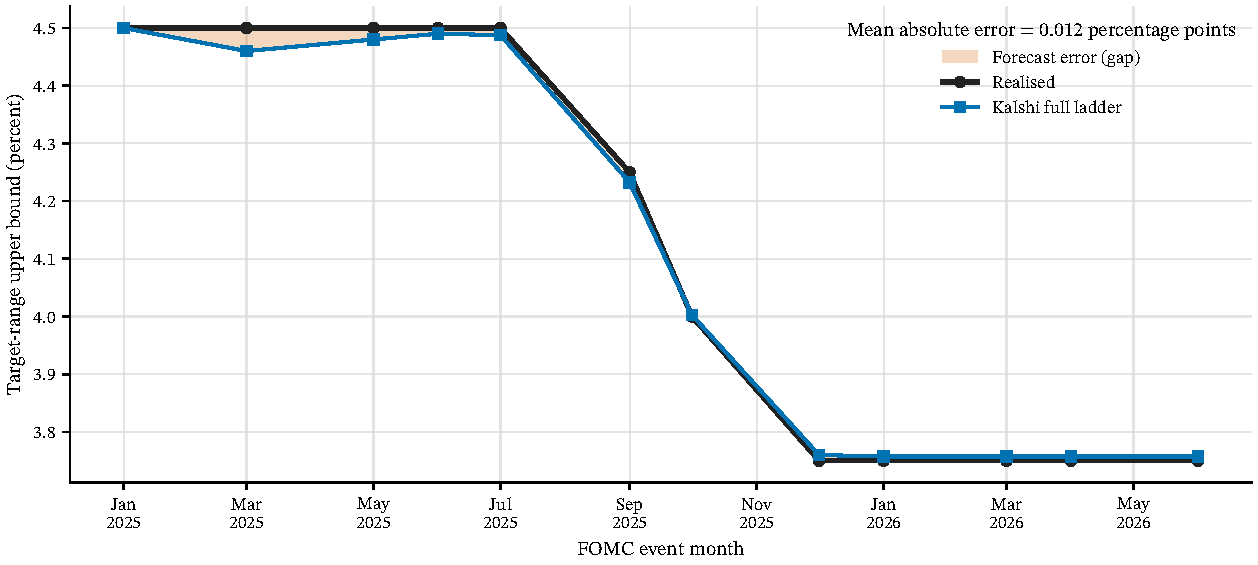
\includegraphics[width=\textwidth]{figures/ffr_h1_kalshi_forecast_error_band.pdf}
    \caption{Terminal full-ladder Kalshi forecast and realised federal funds
    target-range upper bound, 12 test meetings. Shading is the forecast error.}
    \label{fig:app-ffr-errorband}
\end{figure}

\begin{figure}[H]
    \centering
    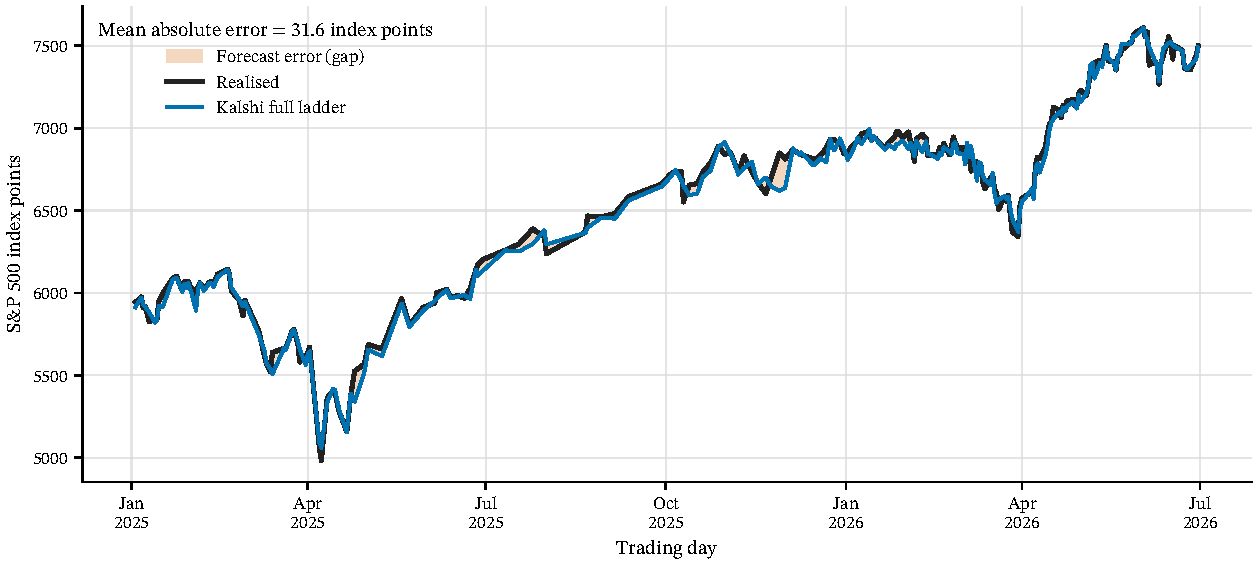
\includegraphics[width=\textwidth]{figures/sp500_h1_kalshi_forecast_error_band.pdf}
    \caption{Terminal full-ladder Kalshi forecast and realised S\&P~500 cash
    close, 229 test days. Shading is the forecast error.}
    \label{fig:app-sp500-errorband}
\end{figure}

\end{document}
